\documentclass[12pt,a4paper]{article}
\usepackage{amsmath,amssymb,amsfonts,amsthm,booktabs,setspace,subcaption,algorithm,algorithmic}
\usepackage{graphicx}
\graphicspath{{../}} 
\usepackage[dvipsnames]{xcolor}
\usepackage{pdflscape}
\usepackage[round]{natbib} 
\usepackage[colorlinks=true,linkcolor=red,citecolor=red,urlcolor=blue]{hyperref}
\bibliographystyle{plainnat}
\defcitealias{ecdc_covid_france_2020}{ECDC,~2020}
\usepackage[margin=2cm]{geometry}
\usepackage[title]{appendix}
\usepackage{multirow}
\usepackage{longtable}
\usepackage{float}
\newcommand{\R}{\mathbb{R}}
\newtheorem{proposition}{Proposition} 
\newtheorem{corollary}{Corollary}
\newtheorem{theorem}{Theorem}
\newtheorem{lemma}{Lemma}
\newtheorem*{remark}{Remark}
\onehalfspacing
\title{\textbf{Peak Prediction Using Quantile Regression and Asymmetric Laplace Noise}}
\title{\textbf{Sequential Estimation of a Peak Location by Quantile Regression: Stabilization and Entry–Exit Intervals}}
%\usepackage{authblk}
%\usepackage{orcidlink} 
\author{}
%\author[1]{Sa\"{i}d Maanan\,\orcidlink{0000-0001-9365-7586}%
%\thanks{Corresponding author: \texttt{maanan.said@gmail.com}}}
%\author[2]{Azzouz Dermoune}
%\author[3]{Daoud Ounaissi}
%\author[4]{Yousri Slaoui}
%\author[1]{Ahmed El Ghini}
%
%\affil[1]{LEAM, Mohammed V University in Rabat,  Morocco}
%\affil[2]{Laboratoire Paul Painlevé, USTL–CNRS–UMR 8524, Lille, France}
%\affil[3]{ESA, Angers, France}
%\affil[4]{Univ. Poitiers, Lab. Math. et Appl., Futuroscope Chasseneuil, France}
%\affil[4]{Dep. of Math. and Stat, Univ. Moncton, Moncton, NB, E1A 3E9, Canada}

\date{}

\begin{document}
\maketitle

\begin{abstract}
	Predicting a peak before it is fully observed matters in epidemiology, energy and finance. We estimate the height, timing and width of a noisy bell-shaped peak with a robust quantile-based method, updated as data arrive. In simulations, the estimated peak date settles on the true date by the peak at low noise, but settles at all in only a third of high-noise series. For noisy series we propose data-driven intervals for the peak date, built from how much successive estimates still move. Such intervals can contain the true date only once the peak is reached; in simulations they always do at low noise, but only 61--89\% do at high noise by the final horizon. For first-wave COVID-19 in China, France and Germany, intervals selected without knowing the peak contained it in 8 of 12 cases ten days later. Forecasters can judge when peak-date predictions are trustworthy.
\end{abstract}

\noindent
\textbf{Keywords:} Peak location estimation; quantile regression; asymmetric Laplace distribution;
sequential estimation; stabilization time; entry--exit intervals; signal-to-noise ratio; COVID-19.\\

\noindent
\textbf{Mathematics subject classification:} 62M10, 62G35, 60G35.


\noindent
\textbf{JEL classification:} C22, C21, C53, I18.

\clearpage

\section{Introduction}
\label{section:1}

Predicting peaks in time series data is important across a wide range of applications involving proactive decision-making, risk management, resource allocation, and disaster preparedness. Examples include anticipating disease outbreaks in epidemiology and peak demand in energy systems. Peak prediction is challenging because observations are affected by noise, and the underlying signal may be difficult to identify from partial observations. Measurement errors and random fluctuations can make the location and amplitude of a peak difficult to estimate before it is fully observed. Moreover, real-world time series may exhibit multiple peaks, irregular peak shapes, or other temporal structures that are not adequately described by simple forecasting models.

Popular forecasting approaches, such as Autoregressive Integrated Moving Average (ARIMA) models and Recurrent Neural Networks (RNNs), can be effective for describing temporal dependence and forecasting general patterns, but they are not specifically designed to estimate the timing and magnitude of a future peak. A model that provides a good overall forecast may not necessarily provide an accurate estimate of the location of a peak. There has also been comparatively little theoretical work devoted specifically to peak prediction in time series. One contribution in this direction is the thesis of~\citet{Tuc20}, which studies the interplay between trend, seasonality, and noise; see also~\citep{YuB2019,See17}.

Our approach builds on the framework developed in~\citet{Der25}. We consider observations available up to a current observation horizon \(T\) and a prescribed search horizon \(h\geq T\). The observations are modeled as a Gaussian-shaped signal with amplitude \(A>0\), peak location \(L\), and spread \(S>0\), corrupted by additive noise. Our objective is to estimate these parameters from the observations available up to time \(T\) and, in particular, to predict the peak location \(L\) before it is fully observed.

Our first contribution is to extend the least-absolute-deviation criterion used in the symmetric case to a general quantile regression criterion indexed by \(\tau\in(0,1)\). As shown in Section~\ref{section:quantile_amplitude}, for fixed location and spread, the amplitude minimizing this criterion is a weighted \(\tau\)-quantile of a transformed version of the observations. The weighted-median estimator is recovered as the special case \(\tau=1/2\). We also examine the behavior of the quantile-based objective in the noise-free setting in Section~\ref{sec:noise-free}.

Our second contribution concerns the noise model. It is well known that
the check loss $\rho_\tau$ is, up to constants, the negative
log-likelihood of the asymmetric Laplace distribution
\citep{Koenker1999,Yu2001}. 
In Section~\ref{sec:symmetric_laplace_estimation}, we use this
correspondence to define a $\tau$-aligned asymmetric Laplace noise
model, $\mathbb P(e(t)<0)=\tau$, calibrate its scale to a prescribed
signal-to-noise ratio, and study how $\tau$ and the SNR affect peak
estimation in a Gaussian-shaped signal.
Section~\ref{sec:parameter_estimation_paths} investigates the evolution of the sequential peak-location estimator as the observation horizon increases. In particular, we study its stabilization time, defined as the first horizon from which the estimated location remains constant over all subsequent horizons, subject to a minimum plateau-length condition.

Our third contribution addresses situations in which the sequential estimate does not stabilize sufficiently early to provide a reliable point prediction. In Section~\ref{sec:entry-exit}, we develop a data-driven construction of candidate entry and exit times based on the oscillations of the sequential peak-location estimates. These times define candidate intervals for the peak region using only the estimation trajectory, without requiring knowledge of the true peak location \(L\).
We also show that the oscillation function has a ladder structure
(Proposition~\ref{prop:ladder}), which links these intervals to
threshold-based entry and exit times and to the stabilization time of
Section~\ref{sec:parameter_estimation_paths}.
We then introduce an operational rule for selecting a candidate interval based on whether it contains the current point estimate. The performance of this procedure is assessed through Monte Carlo simulations, including empirical interval-selection rates and coverage probabilities. The true peak location is used only retrospectively to evaluate the selected intervals; the construction itself does not guarantee a prescribed coverage level.

Finally, we illustrate the methodology using daily COVID-19 case counts during the first wave of the pandemic in China~\citep{Bar20}, France, and Germany.
The real-world application in Section~\ref{sec:covid-real-data} examines the
estimated peak trajectories, the behavior of the proposed entry--exit
construction across several quantile levels, and its comparison with
threshold-based entry and exit times with data-driven thresholds.

The remainder of the paper is organized as follows. Section~\ref{section:quantile_amplitude} introduces the Gaussian peak model and the quantile-based estimation procedure, including the weighted-quantile characterization of the amplitude estimator. Section~\ref{sec:noise-free} examines the quantile-based objective in the noise-free setting. Section~\ref{sec:symmetric_laplace_estimation} introduces the \(\tau\)-aligned asymmetric Laplace noise model and establishes its connection with the quantile loss. Section~\ref{sec:parameter_estimation_paths} studies the stabilization of the sequential peak-location estimator, while 
Section~\ref{sec:entry-exit} develops the candidate entry--exit intervals,
relates them to threshold-based entry and exit times through a ladder
structure of the oscillations (Proposition~\ref{prop:ladder}), and
evaluates the operational selection procedure.
Section~\ref{sec:covid-real-data} presents the real-world COVID-19
application, including comparisons across quantile levels, tables of
estimated peak trajectories, and the entry and exit times obtained with
data-driven thresholds (Section~\ref{subsec:real-entry-eps}).

\section{Quantile-Based Estimation Methodology}
\label{section:quantile_amplitude}

We consider the problem of estimating the amplitude, location, and spread of a unimodal signal corrupted by noise. The model is:
\begin{equation}
	I(t)
	=
	A\exp\left(-\frac{(t-L)^2}{S^2}\right)+e(t),
	\qquad t=1,\ldots,T.
	\label{eq:signal_model}
\end{equation}
where \( A > 0 \) is the amplitude, \( L > 0 \) the peak location, \( S > 0 \) the spread (scale), and \( e(t) \) is additive noise. Given observations \( (I(t))_{t=1}^T \), our goal is to estimate the underlying parameters using quantile regression, i.e., minimizing the asymmetric loss
\begin{equation}
	\rho_\tau(u)
	=
	u\left(\tau-\mathbf{1}_{\{u<0\}}\right).
	\label{eq:check_function}
\end{equation}
for a fixed quantile level \( \tau \in (0,1) \).
We define the quantile objective:
\begin{equation}
	f_\tau(T,a,l,s)
	=
	\frac{1}{T}
	\sum_{t=1}^T
	\rho_\tau
	\left(
	I(t)-a\exp\left(-\frac{(t-l)^2}{s^2}\right)
	\right).
	\label{eq:quantile_objective}
\end{equation}
For fixed candidate values of \( (l,s) \), the optimal amplitude \( a \) minimizes \( a \mapsto f_\tau(T,a,l,s) \). This minimizer is a weighted \(\tau\)-quantile of a transformed version of the data, as described below.

\subsection{Weighted Quantile Estimation of Amplitude}
\label{sec:weighted_median_method}

Let \( w(t) = \exp\left( -\frac{(t - l)^2}{s^2} \right) \) be the weight associated with time point \( t \), and define:
\[
x(t) = I(t) \exp\left( \frac{(t - l)^2}{s^2} \right).
\]
Then the optimal amplitude $a$ is the weighted $\tau$-quantile of
$x(t)$ with weights $w(t)$. The following proposition gives the
corresponding characterization of the weighted quantile as the minimizer
of the weighted quantile loss.
The proof of the following Proposition is the same as in the work of~\citet{Nov20}.
\begin{proposition}
\label{prop:weighted:quantile}
Let \( (x(t), w(t)) \) be a sequence of real values with positive weights \( w(t) > 0 \). Then, for any \( \tau \in (0,1) \), the weighted \( \tau \)-quantile minimizes the weighted quantile loss:
\[
q_\tau = \arg\min_{a \in \mathbb{R}} \sum_{t=1}^T w(t)\,\rho_\tau\bigl(x(t) - a\bigr),
\]
where $\rho_\tau$ is the quantile check function defined in~\eqref{eq:check_function}.
To compute \( q_\tau \), sort the values \( x(t) \) in increasing order, obtaining a permutation \( \pi \) such that
\[
x(\pi(1)) \leq x(\pi(2)) \leq \dots \leq x(\pi(T)).
\]
Define the reordered weights \( w_\pi(t) = w(\pi(t)) \). Let
\[
k = \min \left\{ j \in \{1, \dots, T\} : \sum_{t=1}^j w_\pi(t) \geq \tau \sum_{t=1}^T w(t) \right\}.
\]
Then the weighted \( \tau \)-quantile satisfies \( q_\tau = x(\pi(k)) \).
\end{proposition}


\subsection{Quantile-Based Estimation Procedure}

We define the following steps to jointly estimate the location \( \hat{l}(T) \), amplitude \( \hat{a}(T) \), and spread \( \hat{s}(T) \):

\begin{algorithm}[htbp]
\caption{Quantile-based estimation of peak parameters}
\label{algo:quantile}
\begin{algorithmic}[1]
\REQUIRE Time horizon \( T \), upper bound \( h \ge T \), quantile level \( \tau \in (0,1) \)
\STATE For each candidate \( l \in [1, h] \), find \( s^*(l) = \arg\min_s f_\tau(T, a^*(l,s), l, s) \)
\STATE Set \( \hat{l}(T) = \arg\min_l f_\tau(T, a^*(l,s^*(l)), l, s^*(l)) \)
\STATE Set \( \hat{s}(T) = s^*(\hat{l}(T)) \)
\STATE Set \( \hat{a}(T) = a^*(\hat{l}(T), \hat{s}(T)) \)
\ENSURE Estimated parameters \( (\hat{l}(T), \hat{a}(T), \hat{s}(T)) \)
\end{algorithmic}
\end{algorithm}

\subsection{Remark on Asymmetry and Robustness}

This method generalizes the classic Least Absolute Deviations (LAD) estimator, recovered at \( \tau = 0.5 \). By adjusting \( \tau \), we introduce asymmetry into the estimation loss, enabling the model to better adapt to skewed noise distributions. This makes the approach especially valuable in early-warning systems and epidemic peak detection where overestimation and underestimation have asymmetric consequences.

\section{Quantile-Based Objective Function under Noise-Free Conditions}
\label{sec:noise-free}

We first consider the idealized scenario where the signal is not corrupted by noise. The model of interest is given by
\[
I(t) = A \exp\left( -\frac{(t - L)^2}{S^2} \right), \quad t = 1, \dots, T,
\]
where \( A = 15000 \), \( L = 22 \), \( S = 10 \), and \( T \in \{2, 3, 10, 20, 21\} \). The quantile-based estimation procedure is implemented by minimizing the following objective function~\eqref{eq:quantile_objective}.
The amplitude \( a \) is computed via a weighted \( \tau \)-quantile, as described in Section~\ref{section:quantile_amplitude}.

Since the goal is to predict the location \( L \) of the peak before it becomes observable, we restrict the minimization over candidate peak locations \( l > T \). For each value of \( \tau \in \{0.25, 0.5, 0.75, 0.95\} \), we compute and visualize the objective curve \( l \mapsto f_\tau(T, a(T,l), l, s(T,l)) \) for the selected values of \( T \) (see Figure~\ref{fig:quantile_objective_noise_free}).

\begin{figure}[htbp]
    \centering
    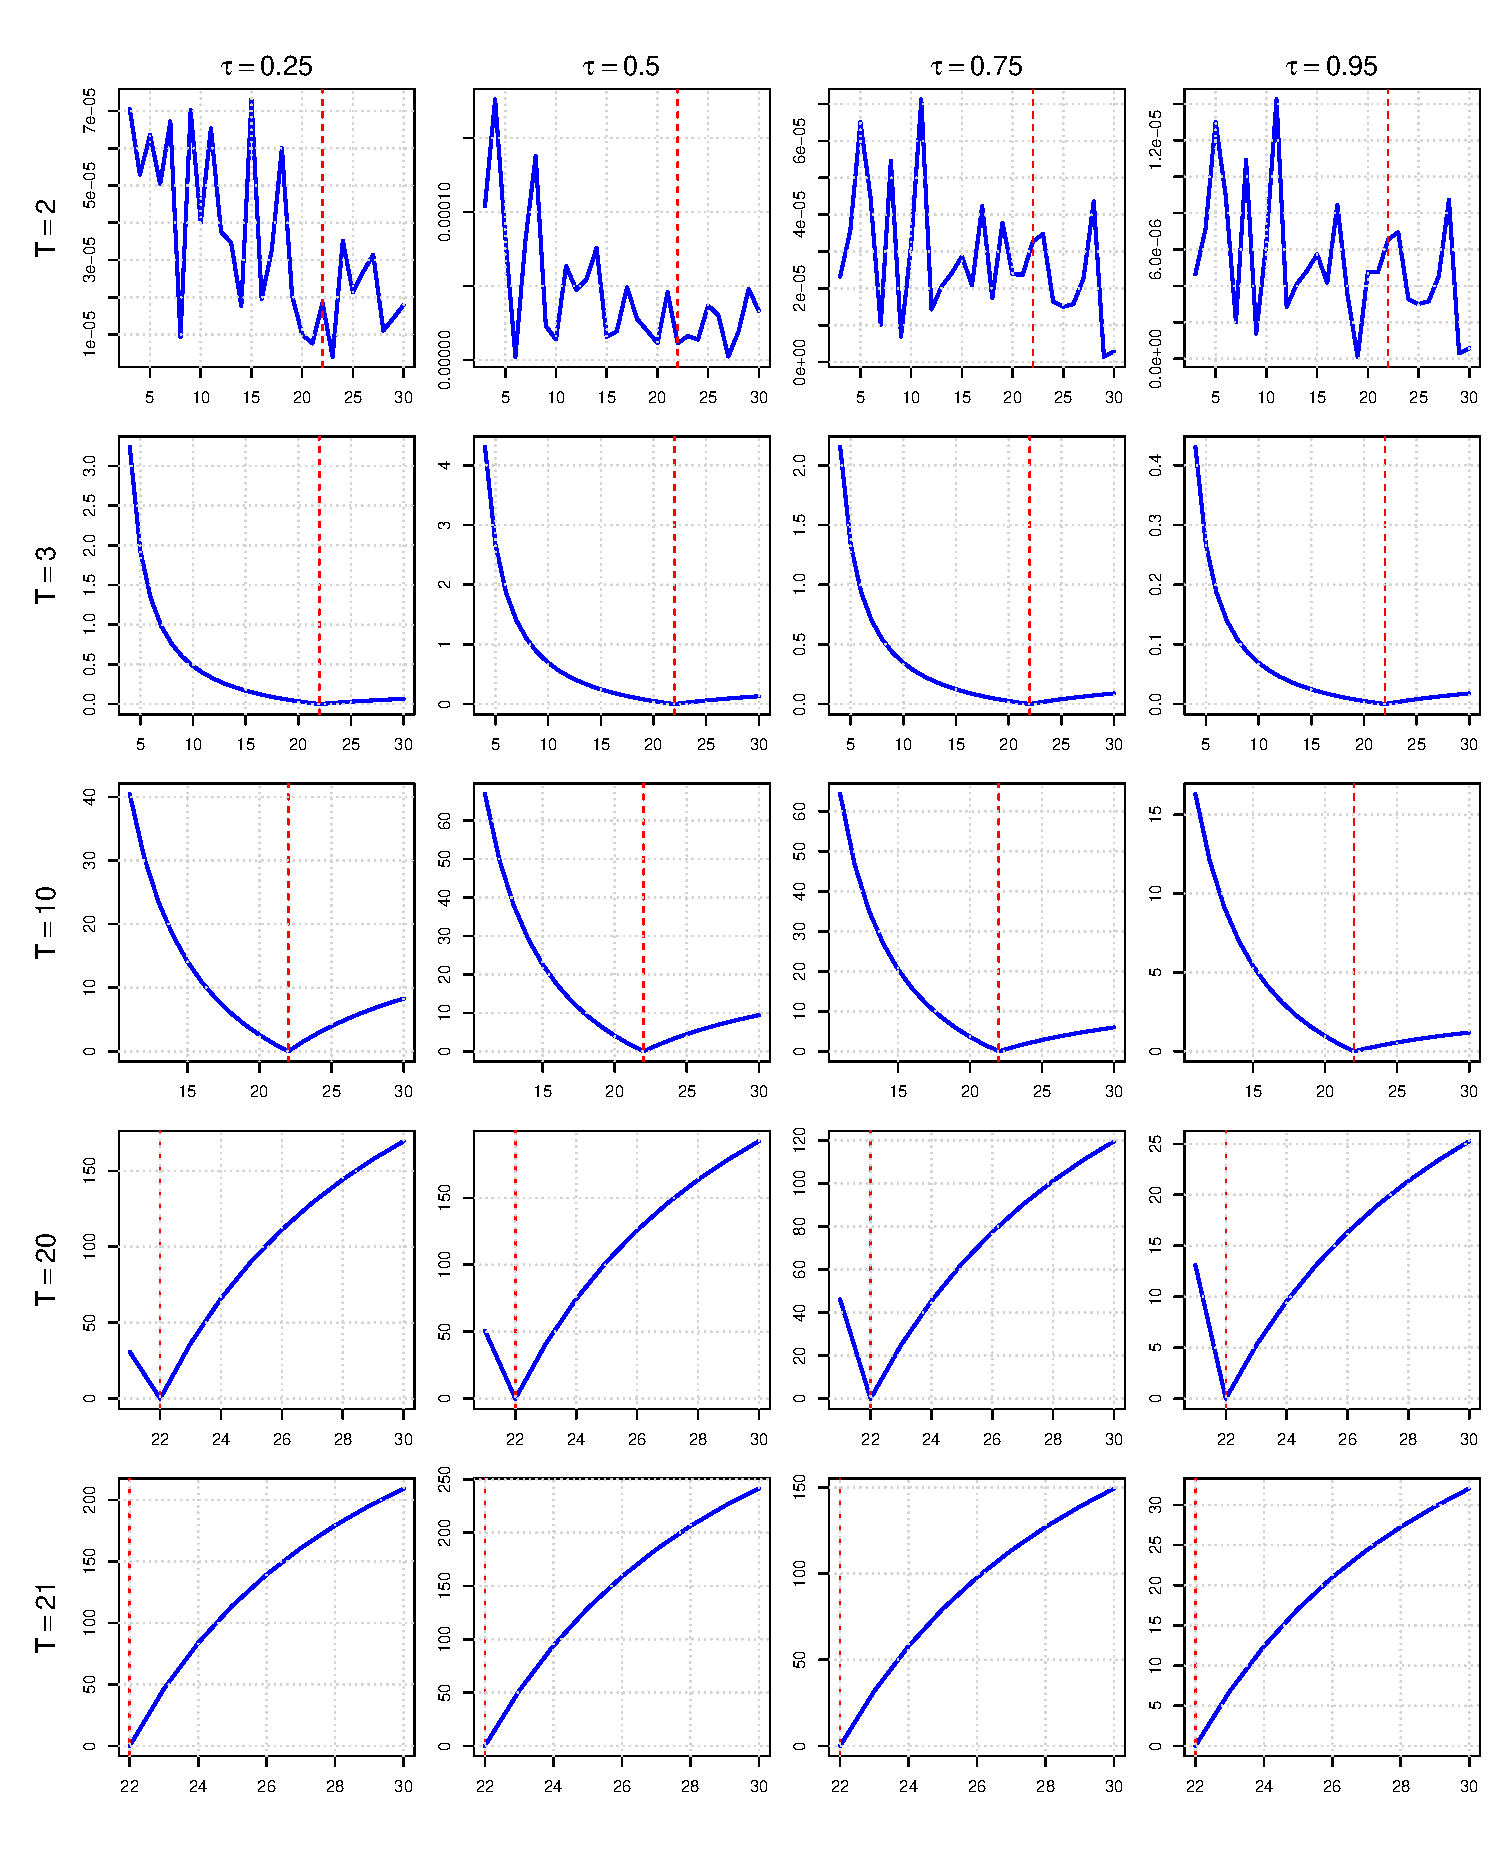
\includegraphics[width=\linewidth]{plot_quantile_all.pdf}
    \caption{Objective function \( l \mapsto f_\tau(T, a, l, s) \) computed for \( \tau \in \{0.25, 0.5, 0.75, 0.95\} \) and \( T \in \{2, 3, 10, 20, 21\} \), under a noise-free signal. The vertical dashed line indicates the true peak location \( L = 22 \), and the search is restricted to values \( l > T \).}
    \label{fig:quantile_objective_noise_free}
\end{figure}

\section{\texorpdfstring{Quantile-Based Estimation with $\tau$-Aligned Noise}{Quantile-Based Estimation with tau-Aligned Noise}}
\label{sec:symmetric_laplace_estimation}

To analyze how quantile-aligned noise affects peak estimation, we introduce a unified noise model based on the \textit{general asymmetric Laplace} (GAL) distribution. This flexible family allows both symmetric and asymmetric noise structures while maintaining the property that the $\tau$-quantile of the noise is at zero.

\subsection{Asymmetric Laplace Noise Aligned with the $\tau$-Quantile}
\label{sec:general_AL_intro}

We consider an asymmetric Laplace distribution parameterized by a location parameter
$m\in\mathbb{R}$, a scale parameter $\lambda>0$, and an asymmetry parameter
$k>0$. Its density is given by
\[
f_{m,\lambda,k}(x)
=
\frac{\lambda}{k+k^{-1}}
\begin{cases}
	\exp\left(\dfrac{\lambda(x-m)}{k}\right), & x<m, \\[8pt]
	\exp\left(-\lambda k(x-m)\right), & x\geq m.
\end{cases}
\]
The parameter $m$ is the mode of the distribution, while $k$ controls its
asymmetry and $\lambda$ controls its concentration.
This is a member of the asymmetric Laplace family; see
\citet{Kotz2001} for its properties.
The distribution function evaluated at the mode is
\[
\mathbb{P}(X<m)
=
\frac{\lambda}{k+k^{-1}}
\int_{-\infty}^{m}
\exp\left(\frac{\lambda(x-m)}{k}\right)\,dx
=
\frac{k^2}{1+k^2}.
\]
Therefore, to align the asymmetric Laplace noise with the $\tau$-quantile
regression criterion, we require
\begin{equation}
	\mathbb{P}(e(t)<0)=\tau,
	\label{eq:tau_alignment}
\end{equation}
and
\(
\tau\in(0,1).
\)
Since the location of the noise can be fixed at zero, we set $m=0$. The
corresponding asymmetry parameter is then determined by
\[
\frac{k^2}{1+k^2}=\tau,
\]
or equivalently,
\begin{equation}
	k
	=
	\sqrt{\frac{\tau}{1-\tau}}.
	\label{eq:asymmetry_parameter}
\end{equation}
Thus, the $\tau$-aligned asymmetric Laplace noise has density
\[
f_{\tau,\lambda}(x)
=
\frac{\lambda}{k+k^{-1}}
\begin{cases}
	\exp\left(\dfrac{\lambda x}{k}\right), & x<0, \\[8pt]
	\exp(-\lambda kx), & x\geq 0,
\end{cases}
\]
where $k$ is given by \eqref{eq:asymmetry_parameter}. 
By construction, the noise satisfies the $\tau$-alignment property
\eqref{eq:tau_alignment}.
In particular, when $\tau=1/2$, we have $k=1$, and the asymmetric Laplace
distribution reduces to the symmetric Laplace distribution centered at zero.
Hence, the symmetric Laplace case is recovered as a special case of the
$\tau$-aligned asymmetric Laplace model.

\subsection{Simulation under Asymmetric Laplace Noise}
\label{subsec:asymmetric_laplace_noise}

We now investigate the behavior of the quantile-based peak estimation procedure when the additive noise follows the $\tau$-aligned asymmetric Laplace distribution introduced in Section~\ref{sec:general_AL_intro}. In the parametrization based on the quantile loss, the density of the noise can be written as
\begin{equation}
	f_{\tau,b}(x)
	=
	\frac{\tau(1-\tau)}{b}
	\exp\left(
	-\frac{1}{b}\rho_\tau(x)
	\right),
	\qquad
	\tau\in(0,1),\quad b>0.
	\label{eq:AL_density}
\end{equation}
where $\rho_\tau$ is the check function defined in~\eqref{eq:check_function}.
Equivalently,
\[
f_{\tau,b}(x)
=
\begin{cases}
	\displaystyle
	\frac{\tau(1-\tau)}{b}
	\exp\left(-\frac{\tau x}{b}\right), & x\geq 0, \\[8pt]
	\displaystyle
	\frac{\tau(1-\tau)}{b}
	\exp\left(\frac{(1-\tau)x}{b}\right), & x<0.
\end{cases}
\]
The normalization follows from
\[
\int_{-\infty}^{+\infty}
\exp\left(-\frac{1}{b}\rho_\tau(x)\right)\,dx
=
\frac{b}{1-\tau}+\frac{b}{\tau}
=
\frac{b}{\tau(1-\tau)}.
\]
Moreover, by construction,
the noise satisfies the $\tau$-alignment property~\eqref{eq:tau_alignment}.
This distribution is directly compatible with the quantile-based estimation criterion. Indeed,
\[
-\log f_{\tau,b}(e)
=
-\log\left(\frac{\tau(1-\tau)}{b}\right)
+
\frac{1}{b}\rho_\tau(e).
\]
This is the standard asymmetric Laplace working likelihood used in
likelihood-based and Bayesian quantile regression
\citep{Koenker1999,Yu2001}.
Therefore, for fixed $\tau$ and $b$, minimizing the negative log-likelihood is equivalent to minimizing the empirical quantile loss. The asymmetric Laplace model thus provides a probabilistic interpretation of the quantile-based peak estimation procedure without introducing a separate estimation criterion.
For the simulation study, the true signal is
\[
I(t)
=
A\exp\left(-\frac{(t-L)^2}{S^2}\right),
\]
with
$A=1,$
$L=22,$
$S=10.$
Since the maximum amplitude of the Gaussian signal is
\(
\max_t I(t)=A,
\)
we define the signal-to-noise ratio as the ratio between the peak
amplitude of the signal and the standard deviation of the noise:
\begin{equation}
	\mathrm{SNR}
	=
	\frac{A}{\sqrt{\operatorname{Var}(e(t))}}.
	\label{eq:SNR_definition}
\end{equation}
In the simulations, we set
\(
\mathrm{SNR}=1000.
\)
For each
\(
\tau\in\{0.25,0.5,0.75,0.95\},
\)
the corresponding asymmetric Laplace noise is generated with asymmetry
parameter~\eqref{eq:asymmetry_parameter}. Thus, the noise variance is
calibrated according to
\begin{equation}
	\operatorname{Var}(e(t))
	=
	\left(\frac{A}{\mathrm{SNR}}\right)^2.
	\label{eq:SNR_condition}
\end{equation}
For the $\tau$-aligned asymmetric Laplace distribution, this variance is
\begin{equation}
	\operatorname{Var}(e(t))
	=
	b^2
	\frac{\tau^2+(1-\tau)^2}
	{\tau^2(1-\tau)^2}.
	\label{eq:AL_variance}
\end{equation}
Combining~\eqref{eq:SNR_condition} and~\eqref{eq:AL_variance} gives
\begin{equation}
	b
	=
	\frac{A}{\mathrm{SNR}}
	\frac{\tau(1-\tau)}
	{\sqrt{\tau^2+(1-\tau)^2}}.
	\label{eq:scale_calibration}
\end{equation}
For each $\tau$, the objective function
$l\mapsto f_\tau(T,a,l,s)$ is evaluated for the time horizons
\(
T\in\{4,6,8,9,10\}.
\)
For each candidate peak location $l$, the scale parameter $s$ is optimized over the prescribed interval, and the amplitude $a$ is determined as the weighted $\tau$-quantile described in Section~\ref{sec:weighted_median_method}. The resulting objective profiles are then compared across the different values of $\tau$.
The resulting profiles are displayed in Figure~\ref{fig:asymmetric_laplace_loss_profiles}. The true peak location $L=22$ is marked by a vertical dashed line. Each panel corresponds to a different pair $(T,\tau)$, and the curves show the behavior of the quantile-loss objective across candidate peak locations.

\begin{figure}[htbp]
	\centering
	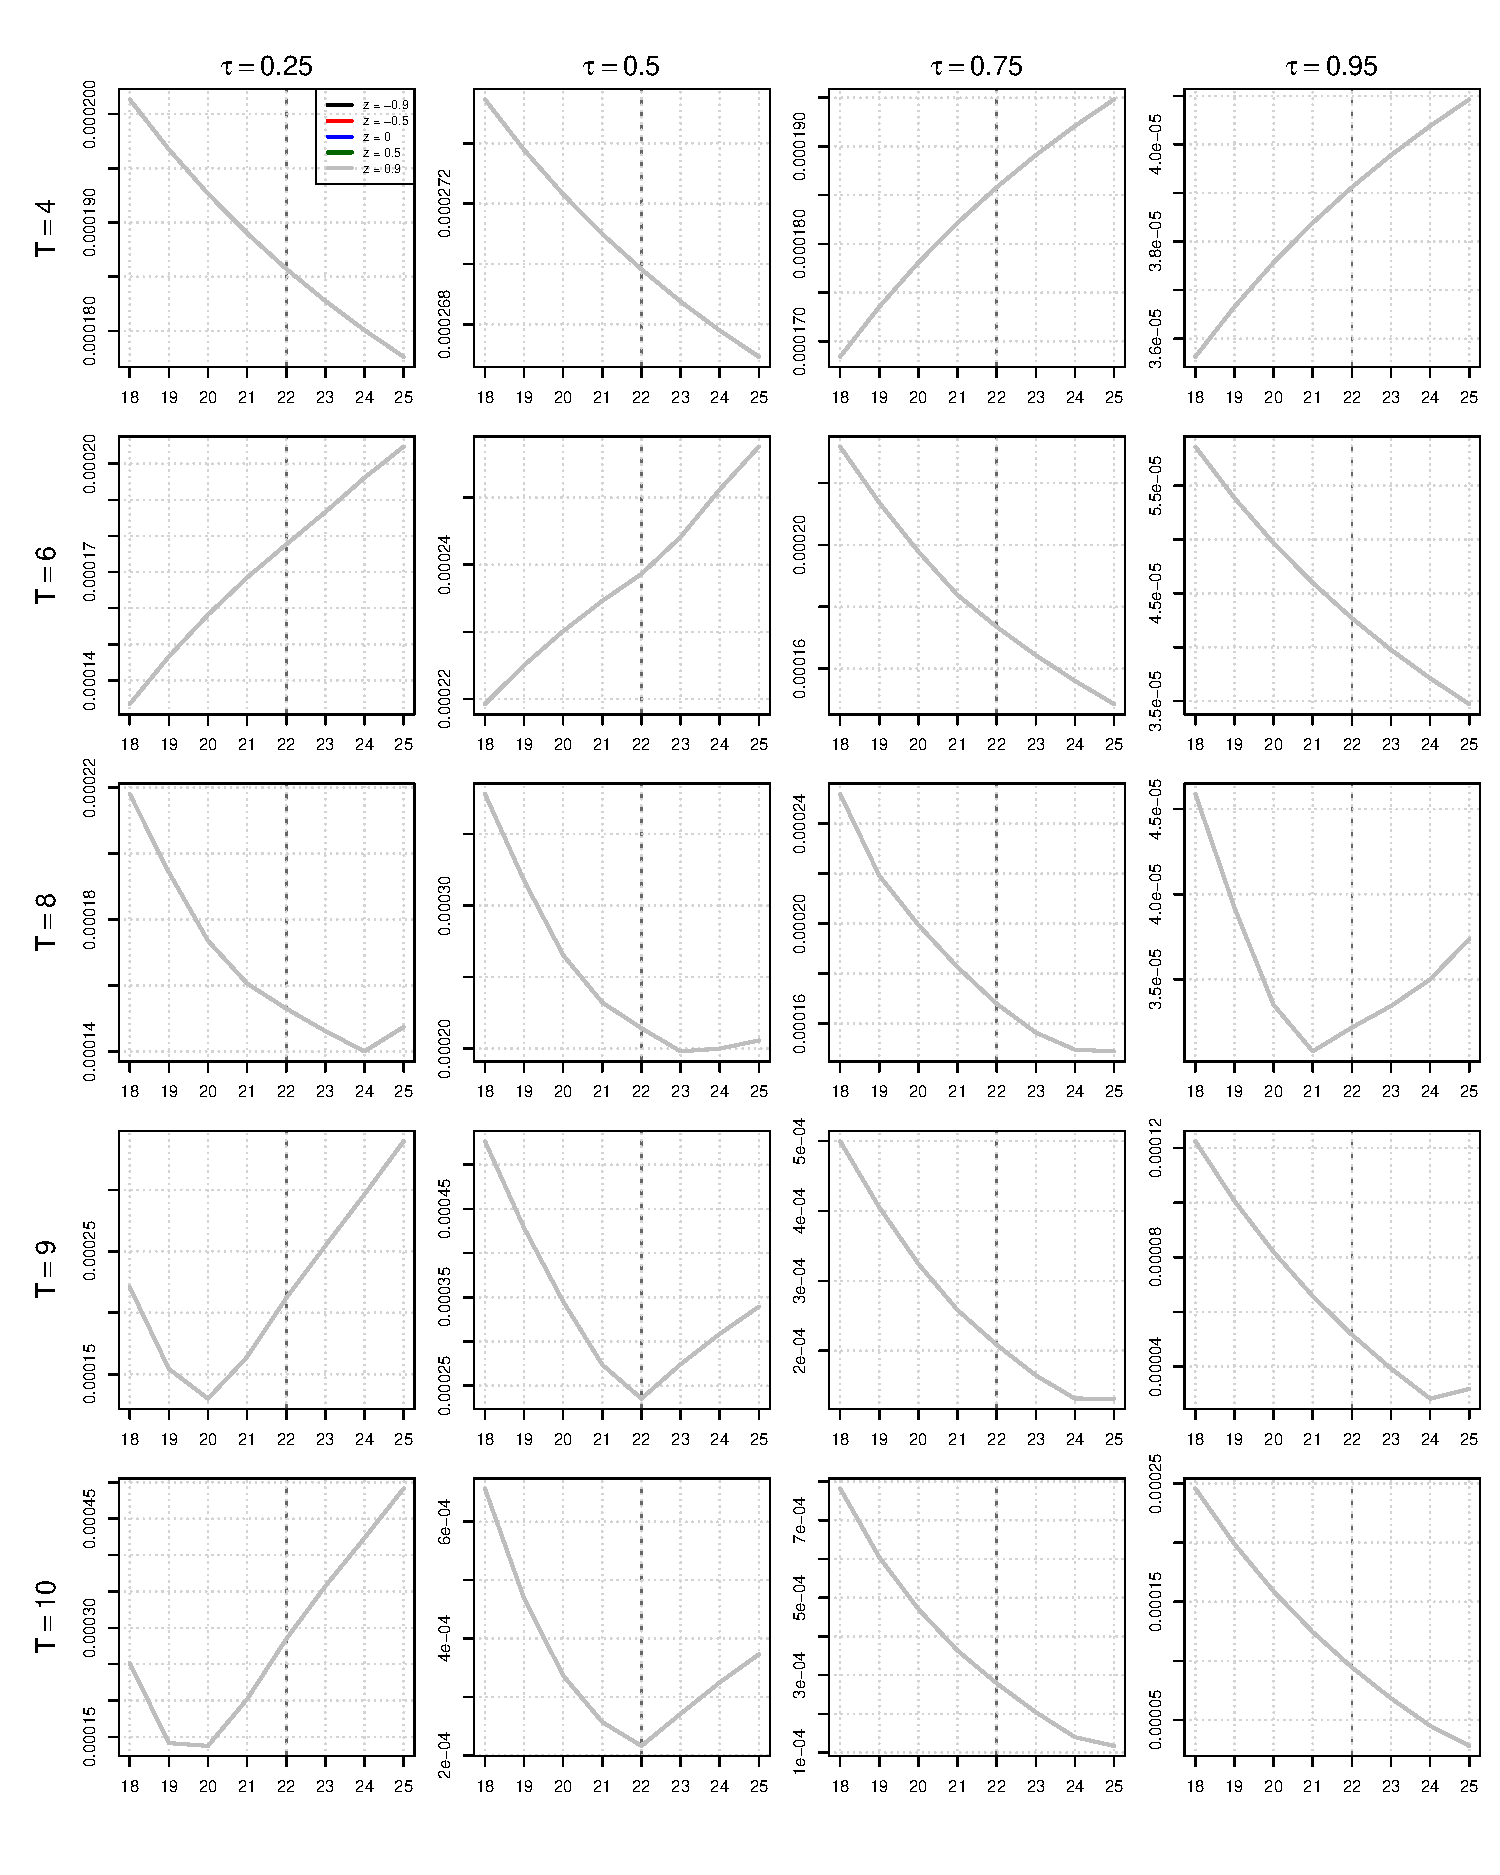
\includegraphics[width=\linewidth]{figure2_asymmetric_laplace_all_tau_T.pdf}
	\caption{Objective function profiles $l\mapsto f_{\tau}(T,a,l,s)$ under \emph{asymmetric Laplace} noise for all combinations of $\tau\in\{0.25,0.5,0.75,0.95\}$ (columns) and $T\in\{4,6,8,9,10\}$ (rows). Each sub-figure shows the loss function for a specific $T$ and $\tau$ pair, with the dashed vertical line indicating the true peak location $L=22$.}
	\label{fig:asymmetric_laplace_loss_profiles}
\end{figure}

\section{Stabilization of the Sequential Estimator}
\label{sec:parameter_estimation_paths}

We study how the estimated peak location $\hat l(T)$ evolves as the
observation horizon $T$ increases. We use the model~\eqref{eq:signal_model}
with $h=30$, $A=1$, $L=22$, $S=10$, $\tau$-aligned asymmetric Laplace
noise (Section~\ref{sec:general_AL_intro}), and
$\mathrm{SNR}\in\{1000,100,1\}$. At each $T\in\{4,\dots,h\}$,
$(\hat l(T),\hat a(T),\hat s(T))$ minimizes the objective
\eqref{eq:quantile_objective}; only $\hat l(T)$ is considered below.

\subsection{Stabilization time}

We define the stabilization time of the path $T\mapsto\hat l(T)$ as
\[
T^{*}
=
\min\{T\in\{4,\dots,h\}:\ \hat l(u)=\hat l(T)\ \text{for all }u\in\{T,\dots,h\}\},
\]
the first horizon from which the estimate no longer changes. This definition
does not use $L$. To exclude a trivial plateau reduced to the last horizon(s),
we require the plateau to contain at least $m=3$ horizons, $h-T+1\ge m$, and
set $T^{*}=\infty$ otherwise. In simulations, where $L$ is known, we also
record whether the plateau value equals $L$, that is, $\hat l(T^{*})=L$.

\subsection{Large and moderate signal-to-noise ratio}

For $\mathrm{SNR}=1000$ and $\mathrm{SNR}=100$, the estimated peak location $\hat l(T)$ reaches a plateau whose value equals $L$ in all replicates. The stabilization time satisfies $T^*\leq L$ in all replicates at $\mathrm{SNR}=1000$ and in $99\%$ of replicates at $\mathrm{SNR}=100$. For $\tau=0.50$ and $M=200$ independent replicates, Table~\ref{tab:tstar} reports median stabilization times of $12$ and $18$, respectively.
In the single realization used in
Section~\ref{subsec:entry-exit-simulation} (seed $280$, $\tau=0.50$),
$T^{*}=9$ at $\mathrm{SNR}=1000$. In these regimes the point estimate
identifies $L$ after a short transient, and $T^{*}$ plays the role of an entry
time. No exit time is needed.

\subsection{Small signal-to-noise ratio}

For $\mathrm{SNR}=1$, the path rarely settles. In the same experiment
($\tau=0.50$, $M=200$), a plateau of at least $m=3$ horizons exists in only
$34\%$ of the replicates ($T^{*}<\infty$), with median $T^{*}=27$, and
$T^{*}>L$ or $T^{*}=\infty$ in $93\%$ of them. The plateau value equals $L$
in only $4.5\%$ of all replicates (about $13\%$ of those with a plateau).
Without the minimal length ($m=1$), $T^{*}$ is always finite, with median
$30=h$, because the last horizon is a trivial plateau; then $\hat l(T^{*})=L$
in $13.5\%$ of the replicates. Figure~\ref{fig:tstar_examples} shows two
replicates: one with finite $T^{*}=24$ and one with $T^{*}=\infty$. In
this regime the path alone does not indicate when its current value can be
trusted. This motivates the entry times, exit times and the data-driven
interval defined in Section~\ref{subsec:oscillations} onward, which are
studied for $\mathrm{SNR}=1$ in Section~\ref{subsec:entry-exit-simulation}.
In the finite example the estimate equals $L$ at $T=22$ but leaves it at
$T=23$, so a single hit of $L$ does not indicate stabilization.

\begin{table}[htbp]
	\centering
	\caption{Stabilization time $T^{*}$ (plateau of at least $m=3$ horizons)
		for $\tau=0.50$, based on $M=200$ replicates. Median $T^{*}$ is
		computed over replicates with finite $T^{*}$; $T^{*}=\infty$ is
		counted as $T^{*}>L$. The last column is the proportion of all
		replicates for which $T^{*}<\infty$ and $\hat l(T^{*})=L$.}
	\label{tab:tstar}
	\begin{tabular}{ccccc}
		\toprule
		SNR & median $T^{*}$ & $\mathbb P(T^{*}<\infty)$
		& $\mathbb P(T^{*}>L)$ & $\mathbb P(T^{*}<\infty,\ \hat l(T^{*})=L)$ \\
		\midrule
		$1000$ & $12$ & $1.00$ & $0.00$ & $1.00$ \\
		$100$  & $18$ & $1.00$ & $0.01$ & $1.00$ \\
		$1$    & $27$ & $0.34$ & $0.93$ & $0.045$ \\
		\bottomrule
	\end{tabular}
\end{table}

\begin{figure}[htbp]
	\centering
	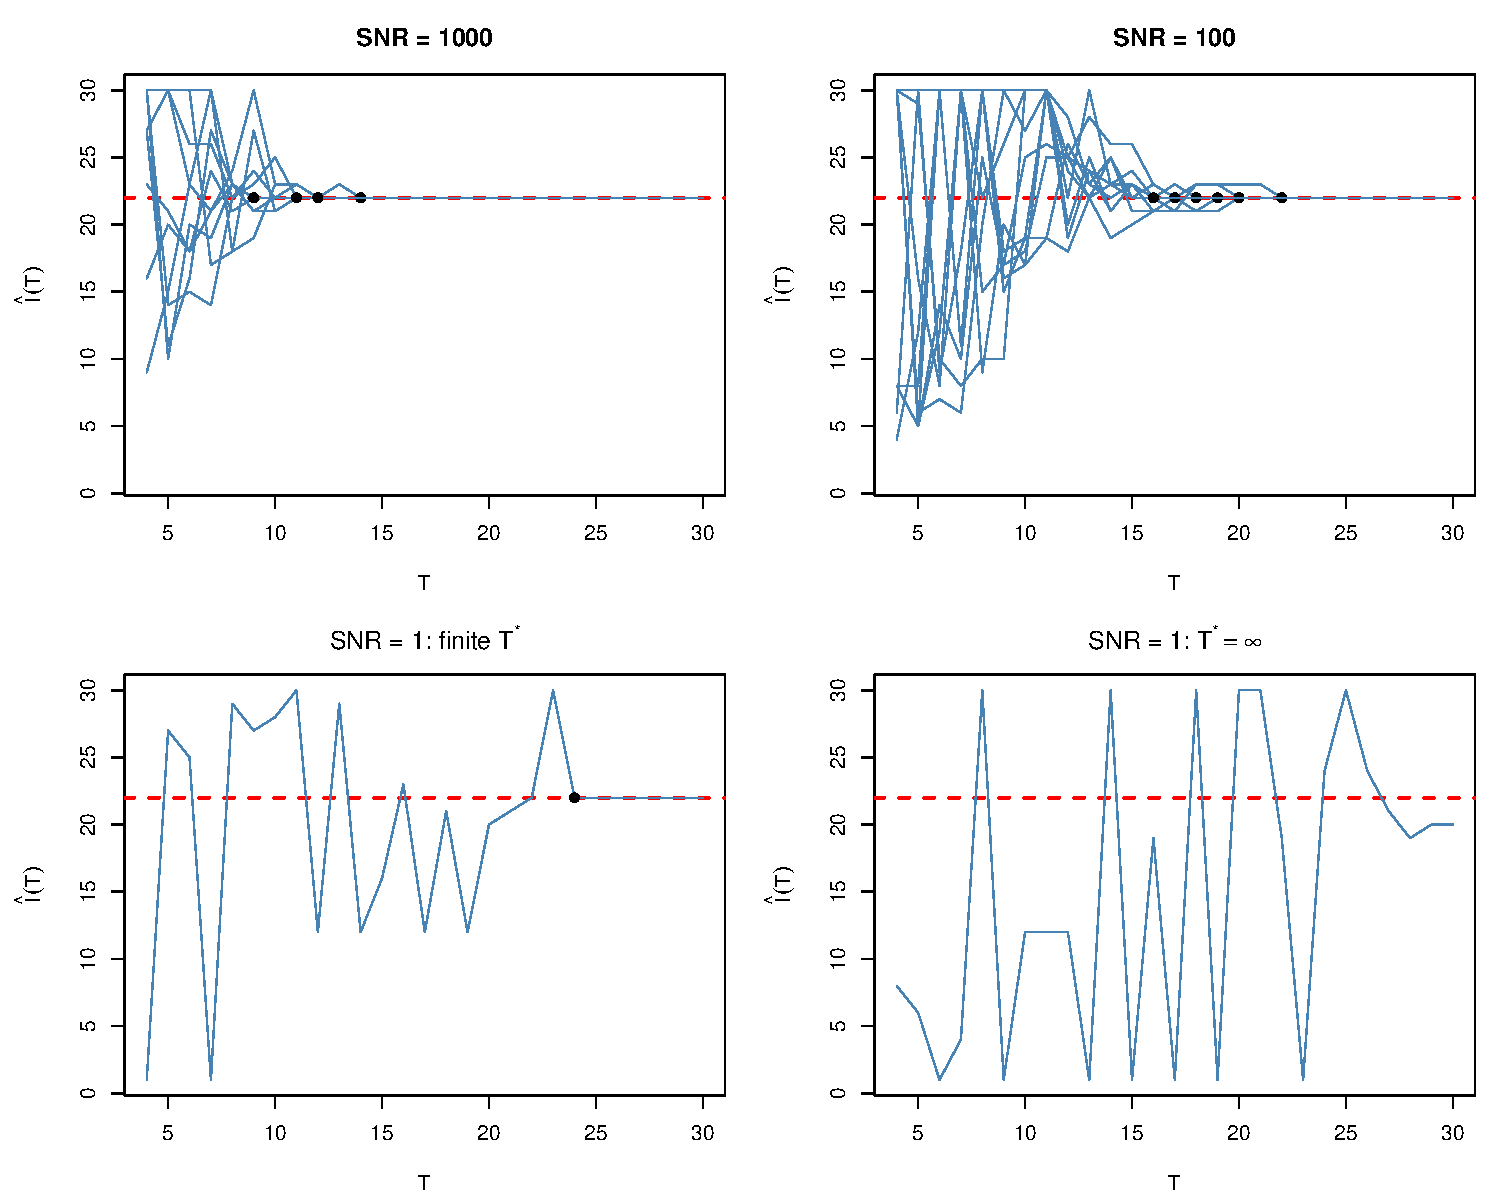
\includegraphics[width=\textwidth]{fig_tstar_examples.pdf}
	\caption{Trajectories $T\mapsto\hat l(T)$ for $\tau=0.50$. Top: ten
		replicates at $\mathrm{SNR}=1000$ and $\mathrm{SNR}=100$. Bottom
		($\mathrm{SNR}=1$): a replicate with finite $T^{*}=24$ (the smallest
		finite value among replicates whose plateau equals $L$), and a replicate
		with $T^{*}=\infty$ (no plateau of at least three horizons). The dashed
		line is $L=22$ and black dots mark $T^{*}$.}
	\label{fig:tstar_examples}
\end{figure}

\section{Entry and Exit Times of the Peak Region}
\label{sec:entry-exit}

The sequential estimation procedure introduced in the preceding sections provides, for each observation horizon \(T\), an estimate \(\hat{l}(T)\) of the peak location. Here, \(T\) denotes the current observation horizon, so that the estimator is constructed using only the observations available on \([1,T]\), while the candidate peak location is searched over the fixed horizon \([1,h]\), with \(T \le h\) and \(L<h\). The case \(T=h\) corresponds to the full-sample estimator and is used in the real-data application of Section~\ref{sec:covid-real-data}.
Thus, although only the observations \(1,\ldots,T\) are used in the estimation, the estimator may identify a peak location beyond the current observation horizon \(T\). For notational simplicity, we write \(\hat{l}(T)\) instead of \(\hat{l}(T,h)\) when the horizon \(h\) is fixed.

The stabilization time defined in Section~\ref{sec:parameter_estimation_paths} characterizes the first horizon from which the estimated peak location remains constant over all subsequent horizons, subject to the minimum plateau-length condition introduced there. In this section, we introduce a complementary construction based on the oscillations of the estimated peak location. This construction aims at identifying candidate time intervals describing the region in which the estimated peak location becomes stable, through a data-driven time of entry and a time of exit.

The operational construction is based only on the sequential estimation trajectory
\(
T\longmapsto\hat{l}(T).
\)
The true peak location \(L\) is not required to construct the candidate entry and exit times. In the simulation study, where \(L\) is known, it is used only for an ex post assessment of whether a candidate peak region contains the true peak.

\subsection{Oscillations of the estimated peak location}
\label{subsec:oscillations}

We fix a sufficiently large horizon \(h\) such that the true peak location satisfies
\(L<h\). For each observation horizon \(T\leq h\), the sequential estimator \(\hat{l}(T)\) is constructed using only the observations available on \([1,T]\), while the candidate peak location is searched over \([1,h]\).
To characterize the temporal stability of the estimated peak location using only the information available at the current observation horizon \(T\), we consider the oscillations of the estimation path over intervals contained in the observed time range \([1,T]\). For two times \(t\) and \(T\) satisfying
\(
T_0\leq t\leq T\leq h,
\)
we define the oscillation of the estimated peak location over the interval \([t,T]\) by
\begin{equation}
	\omega_l(t,T)
	=
	\max_{t\leq t_1,t_2\leq T}
	\left|
	\hat{l}(t_1)-\hat{l}(t_2)
	\right|.
	\label{eq:local_oscillation}
\end{equation}
Thus, \(\omega_l(t,T)\) measures the largest variation of the estimated peak location over the observed interval \([t,T]\). In particular,
\(
\omega_l(T,T)=0.
\)
For a fixed observation horizon \(T\), the function
$t\longmapsto\omega_l(t,T),$
with
$T_0\leq t\leq T,$
is non-increasing. Indeed, if \(t_1<t_2\leq T\), then
\(
[t_2,T]\subset[t_1,T],
\)
and consequently
\(
\omega_l(t_2,T)\leq\omega_l(t_1,T).
\)
The strict decreases of this sequence identify the times at which the oscillation level changes when the starting point of the observed interval is moved forward.

\subsection{Strict-decrease points of the retrospective oscillation}
\label{subsec:strict-decrease-points}

For a fixed observation horizon \(T\leq h\), consider the non-increasing sequence
$t\longmapsto\omega_l(t,T),$
with 
$t\in\{T_0,\ldots,T\}.$
We call an observation time \(t<T\) a \emph{strict-decrease point} of the retrospective oscillation if
\[
\omega_l(t,T)>\omega_l(t+1,T).
\]
We order the strict-decrease points in decreasing order. Thus, if
\(
t_3<t_2<t_1<T
\)
are the strict-decrease points, then
\(
t_1>t_2>t_3.
\)
The intervals between consecutive strict-decrease points correspond to constant plateaus of the non-increasing sequence \(t\mapsto\omega_l(t,T)\). More precisely, if \(U>V\) are two consecutive strict-decrease points, then
\[
\omega_l(t,T)=\omega_l(U,T),
\qquad
t\in\{V+1,\ldots,U\}.
\]
Thus, for each current observation horizon \(T\), the strict-decrease points characterize the successive decreases of the retrospective oscillation computed using only the observations available on \([1,T]\).

\subsection{Construction of the candidate exit times}
\label{subsec:candidate-exit-times}

For each current observation horizon \(T\leq h\), the candidate exit times are defined from the strict-decrease points of the sequence
\(
t\longmapsto\omega_l(t,T).
\)
We set
\(
T_{\mathrm{exit}}^{(0)}(T)=T,
\)
and let
\(
T_{\mathrm{exit}}^{(1)}(T)>
T_{\mathrm{exit}}^{(2)}(T)>
\cdots
\)
denote the strict-decrease points of \(t\mapsto\omega_l(t,T)\) that are strictly smaller than \(T\), ordered in decreasing order.
For example, if the strict-decrease points are
\(
t_3<t_2<t_1<T,
\)
then
\[
T_{\mathrm{exit}}^{(1)}(T)=t_1,\qquad
T_{\mathrm{exit}}^{(2)}(T)=t_2,\qquad
T_{\mathrm{exit}}^{(3)}(T)=t_3.
\]
The convention
\(
T_{\mathrm{exit}}^{(0)}(T)=T
\)
provides the initial candidate exit time, for which
\(
\omega_l\left(T_{\mathrm{exit}}^{(0)}(T),T\right)
=
\omega_l(T,T)
=
0.
\)
For each candidate index \(k\geq0\), we define the corresponding oscillation level by
\[
\epsilon'_k(T)
=
\omega_l\left(
T_{\mathrm{exit}}^{(k)}(T),T
\right).
\]
Thus, for each current observation horizon \(T\), the candidate exit times correspond to the successive strict decreases of the retrospective oscillation, while the associated levels \(\epsilon'_k(T)\) record the oscillation at those candidate exit times.
This construction is based only on the sequential estimation trajectory available up to the current observation horizon \(T\) and does not require knowledge of the true peak location \(L\). Operationally, for each fixed \(T\), the candidate exit times are obtained by scanning the sequence
\(
t\longmapsto\omega_l(t,T)
\)
for its successive strict-decrease points. In numerical implementation, a small tolerance can be used when determining strict decreases.

\subsection{Determination of the entry time}
\label{subsec:entry-time}

For a given current observation horizon \(T\leq h\) and a candidate exit time
\(T_{\mathrm{exit}}^{(k)}(T)\), we first consider all observation times strictly before the candidate exit time. The set
\begin{equation}
	E_k(T)
	=
	\left\{
	t<T_{\mathrm{exit}}^{(k)}(T):
	\omega_l\left(t,T_{\mathrm{exit}}^{(k)}(T)\right)
	\geq
	\epsilon'_k(T)
	\right\},
	\label{eq:stage2_set}
\end{equation}
defines the Stage-2 set. If \(E_k(T)\) is empty, the candidate does not yield a valid entry time. Otherwise, we define
\(
T_k^*(T)=\max E_k(T).
\)
The corresponding oscillation level is
\(
\epsilon_k(T)
=
\omega_l\left(
T_k^*(T),T_{\mathrm{exit}}^{(k)}(T)
\right).
\)
We then consider all observation times \(t<T_{\mathrm{exit}}^{(k)}(T)\) at which the oscillation equals \(\epsilon_k(T)\). The entry time is defined as the smallest such observation horizon:
\begin{equation}
	T_{\mathrm{entry}}^{(k)}(T)
	=
	\min
	\left\{
	t<T_{\mathrm{exit}}^{(k)}(T):
	\omega_l\left(
	t,T_{\mathrm{exit}}^{(k)}(T)
	\right)
	=
	\epsilon_k(T)
	\right\},
	\label{eq:entry-time}
\end{equation}
provided that such an observation time exists.
The width associated with the candidate is
\begin{equation}
	w_k(T)
	=
	T_{\mathrm{exit}}^{(k)}(T)
	-
	T_{\mathrm{entry}}^{(k)}(T).
	\label{eq:peak_region_width}
\end{equation}
The resulting candidate peak region at observation horizon \(T\) is therefore represented by the interval
\[
\mathcal{R}_k(T)
=
\left[
T_{\mathrm{entry}}^{(k)}(T),
T_{\mathrm{exit}}^{(k)}(T)
\right].
\]
All endpoints are determined entirely from the sequential estimation trajectory available up to the current observation horizon \(T\) and from the corresponding retrospective oscillation construction.

\subsection{Threshold-based entry and exit times}
\label{subsec:threshold-entry}
Recall that $\omega_l(t,T)=\max_{t\le u,u'\le T}|\hat l(u)-\hat l(u')|$ is the
oscillation of the path over $[t,T]$ and that $t\mapsto\omega_l(t,T)$ is
non-increasing on $\{T_0,\dots,T\}$.
For thresholds $\varepsilon\ge\varepsilon'\ge0$ let
\[
T_{\mathrm{entry}}(\varepsilon;T)=\min\{t:\omega_l(t,T)\le\varepsilon\},\quad
T_{\mathrm{exit}}(\varepsilon';T)=\min\{t\ge T_{\mathrm{entry}}(\varepsilon;T):\omega_l(t,T)\le\varepsilon'\}.
\]
They are the entry and exit times of \citet{Der25}, except that the
fixed-length window $[t,t+w]$ used there is replaced by the tail $[t,T]$.
Because $\omega_l(\cdot,T)$ is non-increasing and $\varepsilon'\le\varepsilon$,
\[
T_{\mathrm{exit}}(\varepsilon';T)=T_{\mathrm{entry}}(\varepsilon';T)\ \ge\
T_{\mathrm{entry}}(\varepsilon;T):
\]
the exit time is the entry time at the smaller threshold. If
$\varepsilon'=\epsilon'_j$ is a level of the ladder of
Proposition~\ref{prop:ladder} below, it marks the start of rung $j$,
whereas $T_{\mathrm{exit}}^{(k)}(T)=T_{\mathrm{entry}}(\epsilon'_{k-1};T)-1$
is the last horizon of rung $k$.

\begin{proposition}[Ladder structure]\label{prop:ladder}
	Fix $T$. Let $T_{\mathrm{exit}}^{(1)}>\dots>T_{\mathrm{exit}}^{(K)}$ be the
	strict-decrease points of $t\mapsto\omega_l(t,T)$, set
	$T_{\mathrm{exit}}^{(0)}=T$, $\epsilon'_k=\omega_l(T_{\mathrm{exit}}^{(k)},T)$,
	so that $0=\epsilon'_0<\epsilon'_1<\dots<\epsilon'_K$, and use the conventions
	$\epsilon'_{K+1}=\infty$ and $T_{\mathrm{exit}}^{(K+1)}+1=T_0$. Then:
	\begin{enumerate}
		\item[(i)] $\omega_l(t,T)=\epsilon'_k$ for
		$T_{\mathrm{exit}}^{(k+1)}<t\le T_{\mathrm{exit}}^{(k)}$; hence
		$T_{\mathrm{entry}}(\varepsilon;T)=T_{\mathrm{exit}}^{(k+1)}(T)+1$ whenever
		$\epsilon'_k\le\varepsilon<\epsilon'_{k+1}$. In particular
		$T_{\mathrm{entry}}(0;T)=T_{\mathrm{exit}}^{(1)}(T)+1$ is the start of the
		final plateau of $\hat l$.
		\item[(ii)] $T_{\mathrm{exit}}^{(k)}(T)=T_{\mathrm{entry}}(\epsilon'_{k-1};T)-1$
		for $1\le k\le K$.
		\item[(iii)] If $E_k(T)\neq\emptyset$, then
		$T_{\mathrm{entry}}^{(k)}(T)=T_{\mathrm{entry}}\bigl(\epsilon_k(T);T_{\mathrm{exit}}^{(k)}(T)\bigr)$.
		Consequently $T_{\mathrm{entry}}(\epsilon_k(T);T)\ge T_{\mathrm{entry}}^{(k)}(T)$,
		with equality iff $\omega_l\bigl(T_{\mathrm{entry}}^{(k)}(T),T\bigr)\le\epsilon_k(T)$.
		\item[(iv)] For $k=0$: $T_0^{*}=T-1$, $\epsilon_0(T)=|\hat l(T)-\hat l(T-1)|$ and
		$T_{\mathrm{entry}}^{(0)}(T)=T_{\mathrm{entry}}(\epsilon_0(T);T)$. This equals
		$T_{\mathrm{exit}}^{(1)}(T)+1$ if $\hat l(T)=\hat l(T-1)$ and
		$T_{\mathrm{exit}}^{(2)}(T)+1$ otherwise.
	\end{enumerate}
\end{proposition}

\begin{proof}
	(i) $\omega_l(\cdot,T)$ is a non-increasing step function whose strict
	decreases occur at the points $T_{\mathrm{exit}}^{(k)}$, so it equals
	$\epsilon'_k$ on $(T_{\mathrm{exit}}^{(k+1)},T_{\mathrm{exit}}^{(k)}]$. If
	$\epsilon'_k\le\varepsilon<\epsilon'_{k+1}$, the first $t$ with
	$\omega_l(t,T)\le\varepsilon$ is $T_{\mathrm{exit}}^{(k+1)}+1$.
	(ii) Apply (i) with $\varepsilon=\epsilon'_{k-1}$.
	(iii) $t\mapsto\omega_l(t,T_{\mathrm{exit}}^{(k)})$ is non-increasing and equals
	$\epsilon_k$ at $T_k^{*}<T_{\mathrm{exit}}^{(k)}$. Hence
	$\min\{t:\omega_l(t,T_{\mathrm{exit}}^{(k)})\le\epsilon_k\}$ is attained at a
	$t\le T_k^{*}$, where $\omega_l\ge\epsilon_k$, so it equals the minimum in
	\eqref{eq:entry-time}. Moreover $\omega_l(t,T)\ge\omega_l(t,T_{\mathrm{exit}}^{(k)})$
	for $t\le T_{\mathrm{exit}}^{(k)}$, which gives the inequality and the
	equality condition.
	(iv) $E_0(T)=\{t<T\}$, so $T_0^{*}=T-1$ and $\epsilon_0=\omega_l(T-1,T)$;
	(iii) with $k=0$ gives the identity. If $\hat l(T)=\hat l(T-1)$ then
	$\epsilon_0=0=\epsilon'_0$ and (i) gives $T_{\mathrm{exit}}^{(1)}+1$.
	Otherwise $T_{\mathrm{exit}}^{(1)}=T-1$, $\epsilon'_1=\epsilon_0$, and (i) with
	$k=1$ gives $T_{\mathrm{exit}}^{(2)}+1$.
\end{proof}

The proposition ties together three notions of stabilization: the stabilization
time $T^{*}$ of Section~\ref{sec:parameter_estimation_paths}, which equals
$T_{\mathrm{entry}}(0;h)$ when the final plateau has at least $m$ horizons; the
tolerance-based entry time $T_{\mathrm{entry}}(\varepsilon;h)$, $\varepsilon=3,5,15$,
used in Section~\ref{sec:covid-real-data}; and the exit times of the two-stage
construction, by (ii). Apart from $\varepsilon\ge\epsilon'_K$, where
$T_{\mathrm{entry}}(\varepsilon;T)=T_0$, every value of $T_{\mathrm{entry}}(\varepsilon;T)$
is an exit time of the ladder plus one, so choosing $\varepsilon$ amounts to
choosing a rung of the ladder.

\subsection{Construction of a data-driven interval for the peak location}
\label{subsec:entry-exit-simulation}

We illustrate the construction of the entry--exit intervals introduced
in Sections~\ref{subsec:oscillations}--\ref{subsec:entry-time} and
describe how one of these intervals can be selected using only the
observations available at the current horizon. The simulation setting
is the one considered in
Sections~\ref{sec:symmetric_laplace_estimation} and
\ref{sec:parameter_estimation_paths}, with
\(
A=1,
L=22,
S=10,
h=30,
\)
and quantile levels
\(
\tau\in\{0.25,0.50,0.75,0.95\}.
\)
We consider three signal-to-noise ratios,
\(
\mathrm{SNR}\in\{1000,100,1\},
\)
corresponding to large, moderate, and small signal-to-noise regimes,
respectively.
For each current observation horizon $T$, the two-stage procedure
produces a collection of candidate intervals
\[
\mathcal R_k(T)
=
\left[
T_{\mathrm{entry}}^{(k)}(T),
T_{\mathrm{exit}}^{(k)}(T)
\right],
\]
where $k$ indexes the candidate exit times constructed in
Section~\ref{subsec:candidate-exit-times}. The width of candidate
$k$ is
\[
w_k(T)
=
T_{\mathrm{exit}}^{(k)}(T)
-
T_{\mathrm{entry}}^{(k)}(T).
\]
Our objective is to define an operational selection rule that does
not require knowledge of the true peak location $L$.
As shown in Section~\ref{sec:parameter_estimation_paths}, for large
and moderate signal-to-noise ratios, $\hat l(T)$ reaches a plateau
whose value equals $L$ in all replicates, with $T^*\le L$ in all
replicates at $\mathrm{SNR}=1000$ and in $99\%$ of replicates at
$\mathrm{SNR}=100$. In these regimes, the entry time alone is
sufficient for the single-realization examples considered below.
For $\mathrm{SNR}=1$, by contrast, a plateau of at least three
horizons exists in only about one third of the replicates, and
$T^*>L$ or $T^*=\infty$ in most of them. The path alone therefore
does not indicate when its current value can be trusted.
The exit times and the admissible set \(\mathcal K(T)\) introduced below are therefore studied mainly for \(\mathrm{SNR}=1\). The cases \(\mathrm{SNR}=1000\) and \(\mathrm{SNR}=100\) are also reported as high-SNR benchmark cases.

\paragraph{Structure of the candidate intervals.}
For a fixed \(T\), the exit times satisfy
\begin{equation}
	T_{\mathrm{exit}}^{(k+1)}(T)
	<
	T_{\mathrm{exit}}^{(k)}(T),
	\qquad k \geq 0,
	\label{eq:exit-ordering}
\end{equation}
whenever consecutive candidates exist, since the nontrivial exit times are the strict-decrease points of \(t \mapsto \omega_l(t,T)\), ordered from largest to smallest. The candidate intervals are not necessarily nested: in simulations at \(\mathrm{SNR}=1\), consecutive candidates are nested in only about \(30\%\) of the cases and are disjoint in about \(16\)--\(32\%\) of them (details in the supplementary material). The selection rule below uses only \eqref{eq:exit-ordering}.

\paragraph{Operational selection of the interval.}
At a current horizon \(T\), the sequential estimator \(\widehat l(T)\) is available, whereas the true peak location \(L\) is unknown. We therefore select an interval by requiring it to contain the current point estimate. Define the set of admissible candidate indices by
\begin{equation}
	\mathcal K(T)
	=
	\left\{
	k:
	T_{\mathrm{entry}}^{(k)}(T)
	\leq \widehat l(T)
	\leq T_{\mathrm{exit}}^{(k)}(T)
	\right\}.
	\label{eq:admissible-candidates}
\end{equation}
If $\mathcal K(T)$ is nonempty, we select the first admissible candidate:
\begin{equation}
	\widehat k(T)
	=
	\min\mathcal K(T).
	\label{eq:selected-candidate}
\end{equation}
Since the exit times decrease with $k$, this is the admissible candidate with the largest exit time. The rule involves no tie-breaking. The resulting data-driven interval is
\begin{equation}
	\widehat{\mathcal I}(T)
	=
	\left[
	T_{\mathrm{entry}}^{(\widehat k(T))}(T),
	T_{\mathrm{exit}}^{(\widehat k(T))}(T)
	\right].
	\label{eq:selected-peak-interval}
\end{equation}
If $\mathcal K(T)$ is empty, no interval is selected at that horizon, and the procedure can continue as additional observations become available.
We define the first operational selection horizon by
\begin{equation}
	T_{\mathrm{sel}}
	=
	\min\left\{
	T:
	\mathcal K(T)\neq\varnothing
	\right\}.
	\label{eq:T-sel}
\end{equation}
Thus, $T_{\mathrm{sel}}$ is the earliest observation horizon at which the candidate construction produces an interval consistent with the current estimate. It depends only on whether $\mathcal K(T)$ is empty, not on the rule used to choose within $\mathcal K(T)$. Both the selected interval and this selection horizon are computed without using $L$. In contrast, a criterion based on whether the selected interval contains the observed peak $L$ cannot be used operationally and is therefore reserved for retrospective evaluation.

\paragraph{Choice of the selection rule.}
An alternative to \eqref{eq:selected-candidate} is to select the
narrowest admissible candidate,
$\arg\min_{k\in\mathcal K(T)}w_k(T)$. The two rules coincide whenever
$\mathcal K(T)=\{0\}$, which is the case for $\mathrm{SNR}=1000$ and
$\mathrm{SNR}=100$ after $T=22$. For $\mathrm{SNR}=1$, we compared them on
$M=1000$ replicates at $T=30$, among selected intervals
(Table~\ref{tab:rule_comparison}). The narrowest rule gives shorter
intervals but lower coverage. To account for both, we use the interval
score $w+\frac{2}{\alpha}\,\mathrm{dist}(L,\widehat{\mathcal I})$~\citep{Winkler1972,Gneiting2007}, where
$w$ is the width and $\mathrm{dist}$ is the distance from $L$ to the
interval ($0$ if $L$ is inside); lower is better. The first-admissible
rule has the lower score for all four quantile levels and for
$\alpha\in\{0.05,0.10,0.20\}$, at $T=22$, $26$ and $30$, although the
difference is negligible for $\tau=0.95$ at $T=30$ and $\alpha=0.20$.
This is a simulation result for the present model, not a general
property of the rules.

\begin{table}[htbp]
	\centering
	\caption{Selection rules at $\mathrm{SNR}=1$, $T=30$, $M=1000$,
		among selected intervals: coverage ($T_{\mathrm{entry}}\le L\le
		T_{\mathrm{exit}}$), mean width, and interval score
		($\alpha=0.10$). ``First'' is $\min\mathcal K(T)$, ``Narrowest''
		is $\arg\min_{k\in\mathcal K(T)} w_k(T)$.}
	\label{tab:rule_comparison}
	\begin{tabular}{ccccccc}
		\toprule
		& \multicolumn{2}{c}{Coverage} & \multicolumn{2}{c}{Width}
		& \multicolumn{2}{c}{Score} \\
		$\tau$ & First & Narrowest & First & Narrowest & First & Narrowest \\
		\midrule
		$0.25$ & $0.678$ & $0.610$ & $6.35$ & $5.52$ & $25.0$ & $27.8$ \\
		$0.50$ & $0.611$ & $0.552$ & $6.07$ & $5.39$ & $29.3$ & $31.9$ \\
		$0.75$ & $0.667$ & $0.609$ & $6.01$ & $5.33$ & $23.5$ & $25.2$ \\
		$0.95$ & $0.891$ & $0.849$ & $6.33$ & $5.76$ & $10.2$ & $10.8$ \\
		\bottomrule
	\end{tabular}
\end{table}

\paragraph{Numerical results.}
Table~\ref{tab:simulation_est_interval} reports the first operational
selection horizon $T_{\mathrm{sel}}$ and the corresponding selected
interval for each combination of $\tau$ and $\mathrm{SNR}$. The
interval width is
$w_{\widehat k(T_{\mathrm{sel}})}(T_{\mathrm{sel}})$.

\begin{table}[htbp]
	\centering
	\caption{First operationally selected candidate interval for each
		quantile level $\tau$ and signal-to-noise ratio. The selection horizon
		is $T_{\mathrm{sel}}$, and the selected candidate index is
		$\widehat k(T_{\mathrm{sel}})=\min\mathcal K(T_{\mathrm{sel}})$.
		In this realization, $\mathcal K(T_{\mathrm{sel}})$ contains a single
		candidate in every row, so the first-admissible and narrowest rules
		give the same interval. The last column reports the interval width
		$w_{\widehat k(T_{\mathrm{sel}})}(T_{\mathrm{sel}})$.}
	\label{tab:simulation_est_interval}
	\begin{tabular}{cccccccc}
		\toprule
		$\tau$ & SNR
		& $T_{\mathrm{sel}}$
		& $\widehat k(T_{\mathrm{sel}})$
		& $\widehat l(T_{\mathrm{sel}})$ 
		& $T_{\mathrm{entry}}^{(\widehat k(T_{\mathrm{sel}}))}(T_{\mathrm{sel}})$ 
		& $T_{\mathrm{exit}}^{(\widehat k(T_{\mathrm{sel}}))}(T_{\mathrm{sel}})$ 
		& $w_{\widehat k(T_{\mathrm{sel}})}(T_{\mathrm{sel}})$\\ 
		\midrule
		$0.25$ & 1000 & 22 & 0 & 22 & 11 & 22 & 11 \\
		$0.25$ & 100  & 22 & 0 & 22 & 18 & 22 &  4 \\
		$0.25$ & 1    &  6 & 0 &  4 &  4 &  6 &  2 \\
		\midrule
		$0.50$ & 1000 & 22 & 0 & 22 &  9 & 22 & 13 \\
		$0.50$ & 100  & 22 & 0 & 22 & 18 & 22 &  4 \\
		$0.50$ & 1    & 10 & 1 &  8 &  8 &  9 &  1 \\
		\midrule
		$0.75$ & 1000 & 22 & 0 & 22 & 12 & 22 & 10 \\
		$0.75$ & 100  & 22 & 0 & 22 & 16 & 22 &  6 \\
		$0.75$ & 1    & 18 & 0 & 17 & 17 & 18 &  1 \\
		\midrule
		$0.95$ & 1000 & 22 & 0 & 22 & 13 & 22 &  9 \\
		$0.95$ & 100  & 22 & 0 & 22 & 16 & 22 &  6 \\
		$0.95$ & 1    &  9 & 0 &  8 &  8 &  9 &  1 \\
		\bottomrule
	\end{tabular}
\end{table}

For $\mathrm{SNR}=100$ and $\mathrm{SNR}=1000$, the first selected
interval occurs at $T_{\mathrm{sel}}=22$ for all four quantile levels.
For $\mathrm{SNR}=1$, the first selected horizon varies with $\tau$,
taking the values $6$, $10$, $18$, and $9$ for
$\tau=0.25$, $0.50$, $0.75$, and $0.95$, respectively. At
$T_{\mathrm{sel}}$ the set $\mathcal K(T_{\mathrm{sel}})$ is a singleton
in all twelve cases, so the choice of selection rule has no effect on
this table; it matters at later horizons
(Table~\ref{tab:rule_comparison}). The selected
intervals are also substantially narrower in these low-SNR examples.
However, an early and narrow interval need not be close to the true
peak location: in the present realization, the low-SNR intervals
selected at $T_{\mathrm{sel}}$ do not contain $L=22$. This illustrates
that the operational criterion guarantees consistency with
$\widehat l(T)$, not containment of the unknown true peak.
Accordingly, $\widehat{\mathcal I}(T)$ is a data-driven interval
estimate for the peak location. Its construction alone does not
establish a confidence level or guarantee
\[
\mathbb P\!\left\{
L\in\widehat{\mathcal I}(T)
\right\}
\geq 1-\alpha.
\]
To interpret this interval as a confidence interval with nominal
coverage $1-\alpha$, an appropriate coverage result must be established
theoretically or assessed through repeated independent simulation
replicates. The single-realization illustration above is intended to
demonstrate the operational construction and its behavior across
quantile levels and signal-to-noise regimes, rather than to establish
statistical coverage.

\paragraph{Monte Carlo assessment of empirical coverage.}
We next assess the empirical coverage of the operational intervals using repeated independent simulations. For each combination of $\tau\in\{0.25,0.50,0.75,0.95\}$ and $\mathrm{SNR}\in\{1000,100,1\}$, we generate $M=1000$ independent trajectories under the same peak model, with $A=1$, $L=22$, $S=10$, and observation horizon $h=30$. At each available horizon $T$, the operational selection rule defined in \eqref{eq:admissible-candidates}--\eqref{eq:selected-peak-interval} is applied separately to each trajectory. The true peak location $L$ is used only after selection to assess whether the selected interval contains it, with
$L\in\widehat{\mathcal I}(T)$ meaning
$T_{\mathrm{entry}}^{(\widehat k(T))}(T)\le L\le T_{\mathrm{exit}}^{(\widehat k(T))}(T)$.
Let $\widehat{\mathcal I}_m(T)$ denote the selected interval for replicate $m$, when an interval is available. We define the interval-selection rate by
\[
\widehat q_M(T)
=
\frac{1}{M}
\sum_{m=1}^M
\mathbf 1\!\left\{
\widehat{\mathcal I}_m(T) \neq \varnothing
\right\},
\]
and the empirical coverage among selected intervals by
\[
\widehat p^{\,\mathrm{sel}}_M(T)
=
\frac{
	\displaystyle
	\sum_{m=1}^M
	\mathbf 1\!\left\{
	L \in \widehat{\mathcal I}_m(T)
	\right\}
}{
	\displaystyle
	\sum_{m=1}^M
	\mathbf 1\!\left\{
	\widehat{\mathcal I}_m(T) \neq \varnothing
	\right\}
},
\]
provided that at least one interval is selected. We also report the unconditional success proportion
\[
\widehat p^{\,\mathrm{all}}_M(T)
=
\frac{1}{M}
\sum_{m=1}^M
\mathbf 1\!\left\{
L \in \widehat{\mathcal I}_m(T)
\right\}.
\]
Thus, $\widehat p_{\mathrm{all}}(T)$ accounts for both interval-selection failures and selected intervals that do not contain the true peak location. When no interval is selected in any replicate, the conditional coverage is undefined.

Figure~\ref{fig:mc_coverage_selected} displays the empirical coverage among selected intervals as a function of $T$, while Figure~\ref{fig:mc_selection_rate} shows the corresponding interval-selection rates. The results reveal a marked dependence on the signal-to-noise ratio. For $\mathrm{SNR}=1000$, no interval is selected in the simulations for $T<22$, whereas the selection rate and empirical coverage are both equal to one from $T=22$ onward.
For $\mathrm{SNR}=100$, selection is rare at several early horizons. At
$T=22$, the selection rate is between $0.996$ and $1.000$, and all selected
intervals contain $L$. From $T=23$ onward, all simulated trajectories yield a
selected interval, and the empirical coverage is equal to one.
For $\mathrm{SNR}=1000$ and $\mathrm{SNR}=100$ the results do not depend on the selection rule, since $\mathcal K(T)=\{0\}$ in (almost) all replicates after $T=22$.

The low-SNR results are substantially different. At $\mathrm{SNR}=1$, intervals may be selected before $T=22$, but none of the selected intervals at these earlier horizons contains the true peak location in the simulated sample. At $T=22$, the interval-selection rate is between $0.634$ and $0.711$, and the empirical coverage among selected intervals ranges from approximately $0.289$ to $0.418$, depending on $\tau$. Coverage subsequently increases with the observation horizon, although the rate of increase differs across quantile levels. At $T=30$, for example, the empirical coverage is approximately $0.678$, $0.611$, $0.667$, and $0.891$ for $\tau=0.25$, $0.50$, $0.75$, and $0.95$, respectively. At this horizon, the interval-selection rate is at least $0.993$ for all four quantile levels. Hence, the relatively low coverage at small SNR cannot be attributed solely to failures to select an interval.

Table~\ref{tab:mc_coverage_T30} summarizes the selection rates, empirical coverage probabilities, and mean widths at $T=30$. In the high- and medium-SNR settings, all selected intervals contain the true peak location in the simulated replicates. Under low SNR, the empirical coverage is lower, despite the high selection rates. The mean widths also differ across the SNR regimes, illustrating that interval width alone does not determine whether an interval contains the true peak.

These findings provide a simulation-based assessment of the operational procedure under the specified model and parameter settings. In particular, they show that an interval can be selected consistently without necessarily achieving high empirical coverage. The results should therefore be interpreted as empirical coverage probabilities under the considered simulation design, rather than as a general theoretical coverage guarantee.
\begin{table}[htbp]
	\centering
	\small
	\caption{Monte Carlo interval-selection rates, empirical coverage, and mean interval widths at $T=30$, based on $M=1000$ independent replicates and the first-admissible rule \eqref{eq:selected-candidate}. Coverage means $T_{\mathrm{entry}}\le L\le T_{\mathrm{exit}}$. The conditional coverage is calculated among selected intervals, and the unconditional success proportion also accounts for replicates in which no interval is selected.}
	\label{tab:mc_coverage_T30}
	\begin{tabular}{cccccc}
		\toprule
		\(\tau\) & SNR & \(\widehat q_M(30)\) & \(\widehat p^{\,\mathrm{sel}}_M(30)\) & \(\widehat p^{\,\mathrm{all}}_M(30)\) & Mean width \\
		\midrule
		0.25 & 1000 & 1.000 & 1.000 & 1.000 & 18.750 \\
		0.25 &  100 & 1.000 & 1.000 & 1.000 & 12.708 \\
		0.25 &    1 & 0.998 & 0.678 & 0.677 &  6.350 \\
		\midrule
		0.50 & 1000 & 1.000 & 1.000 & 1.000 & 18.283 \\
		0.50 &  100 & 1.000 & 1.000 & 1.000 & 11.992 \\
		0.50 &    1 & 0.993 & 0.611 & 0.607 &  6.066 \\
		\midrule
		0.75 & 1000 & 1.000 & 1.000 & 1.000 & 18.799 \\
		0.75 &  100 & 1.000 & 1.000 & 1.000 & 12.750 \\
		0.75 &    1 & 0.998 & 0.667 & 0.666 &  6.011 \\
		\midrule
		0.95 & 1000 & 1.000 & 1.000 & 1.000 & 19.606 \\
		0.95 &  100 & 1.000 & 1.000 & 1.000 & 14.141 \\
		0.95 &    1 & 1.000 & 0.891 & 0.891 &  6.326 \\
		\bottomrule
	\end{tabular}
\end{table}

\begin{figure}[htbp]
	\centering
	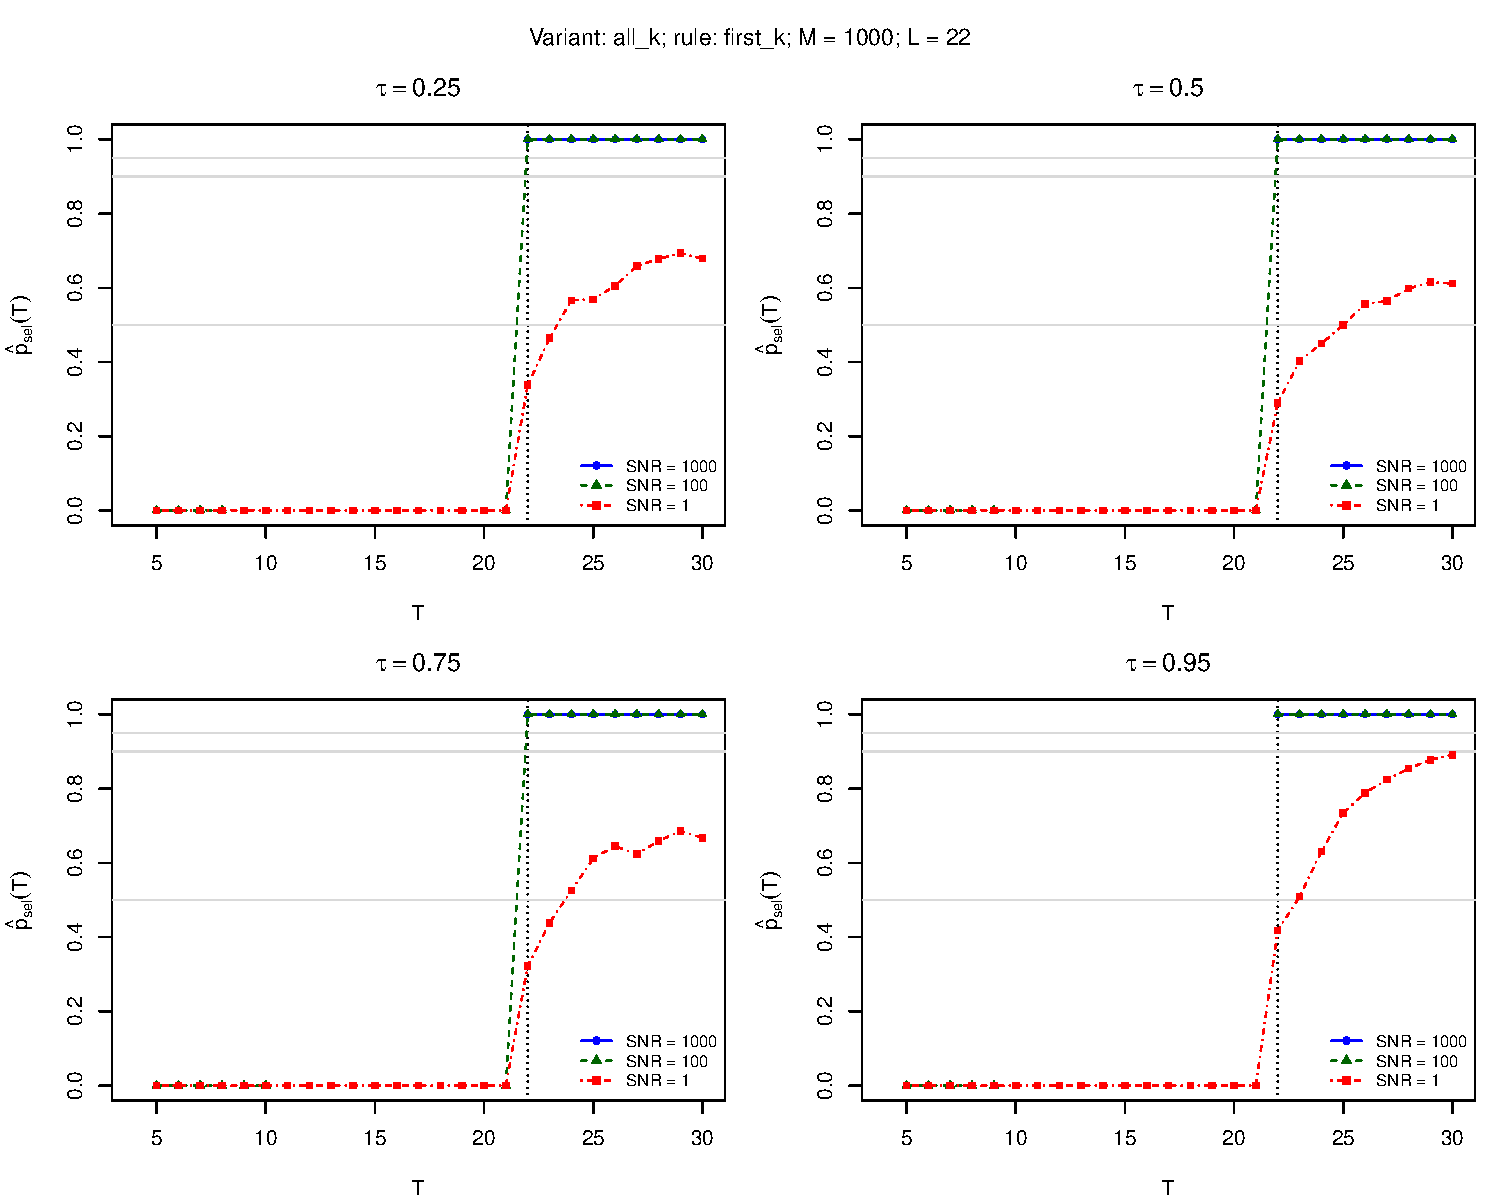
\includegraphics[width=\textwidth]{monte-carlo-coverage-selected.pdf}
	\caption{Empirical coverage ($T_{\mathrm{entry}}\le L\le T_{\mathrm{exit}}$) of the selected operational intervals, using the first-admissible rule, as a function of the observation horizon $T$, based on $M=1000$ independent simulated trajectories for each combination of $\tau$ and SNR. Coverage is calculated conditionally on interval selection. The horizontal axis gives the observation horizon, and each panel corresponds to one quantile level.}
	\label{fig:mc_coverage_selected}
\end{figure}

\begin{figure}[htbp]
	\centering
	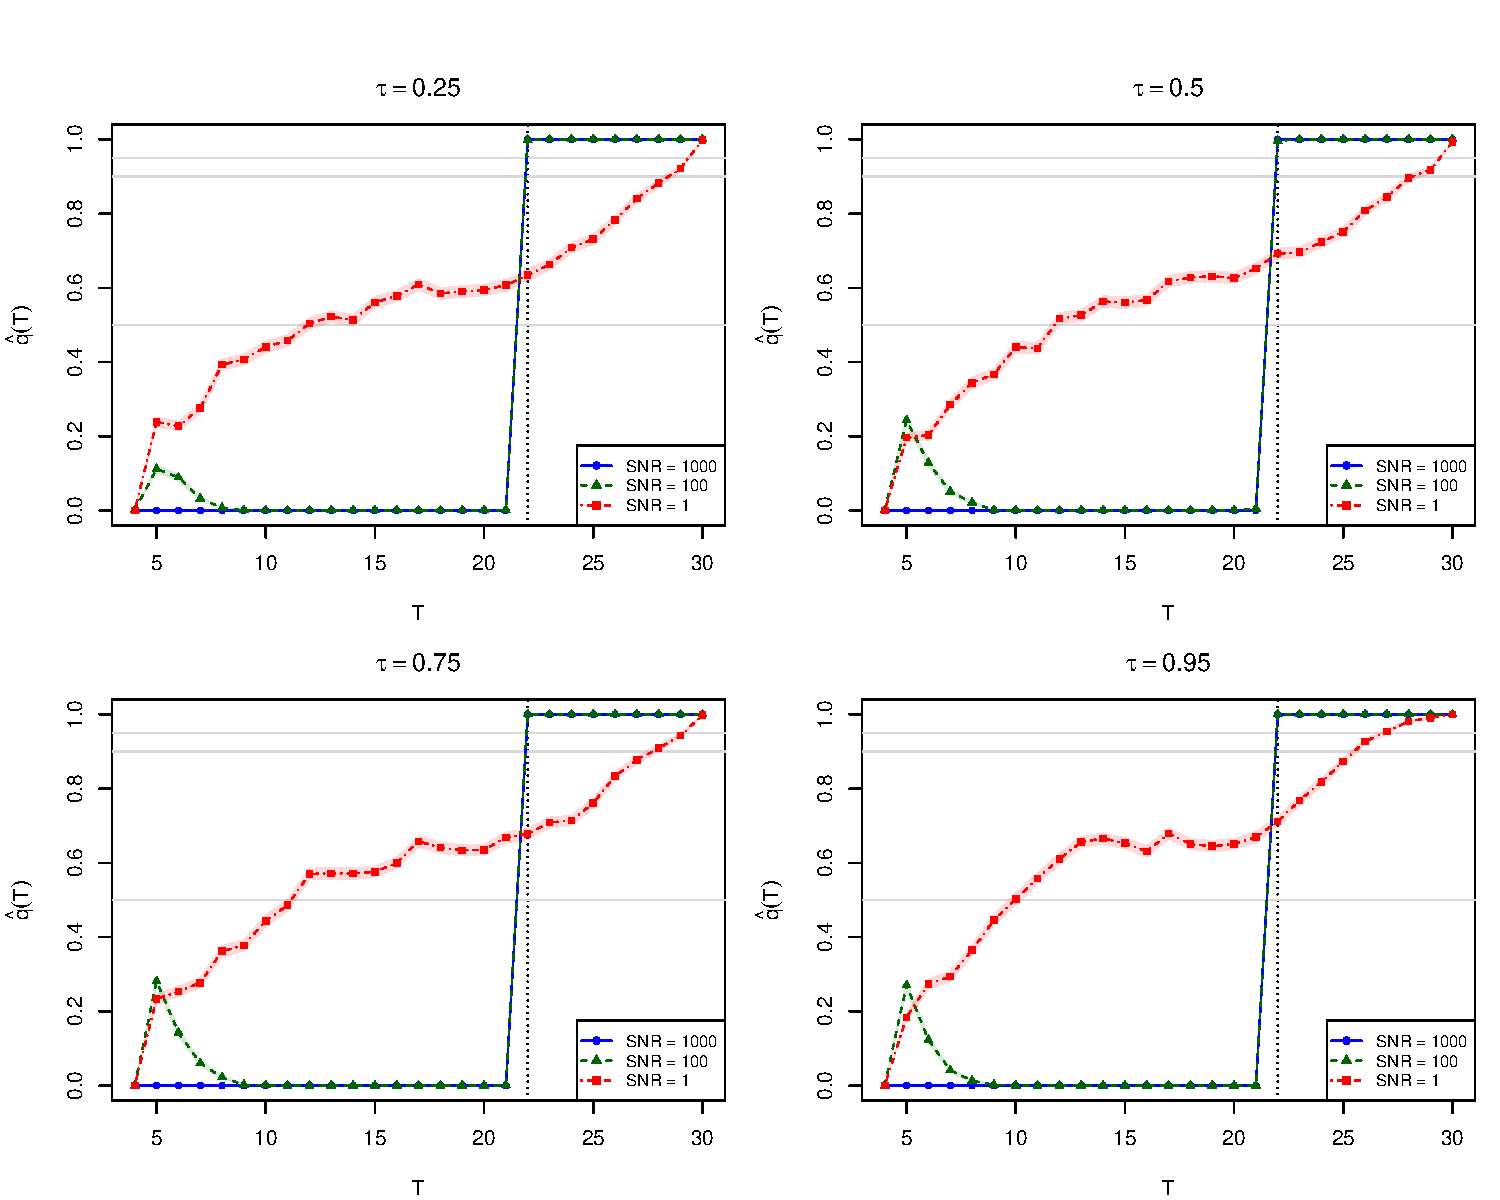
\includegraphics[width=\textwidth]{monte-carlo-interval-selection-rate.pdf}
	\caption{Empirical interval-selection rate as a function of the observation horizon $T$, based on $M=1000$ independent simulated trajectories for each combination of $\tau$ and SNR. The selection rate is the proportion of replicates for which the operational rule selects an interval, and does not depend on the choice of rule within $\mathcal K(T)$. Shaded bands are $\pm$ one Monte Carlo standard error. Each panel corresponds to one quantile level.}
	\label{fig:mc_selection_rate}
\end{figure}

\section{Real-World Application: COVID-19 Case Study}
\label{sec:covid-real-data}

We now demonstrate the application of our quantile-based peak estimation
framework to real-world data. We focus on the daily confirmed COVID-19
cases in China, France, and Germany. Figure~\ref{fig:covid-1x3} displays
the daily case series for these three countries. 
The Chinese series is obtained from the Johns Hopkins University Center for Systems Science and Engineering (JHU CSSE) feed via the \texttt{COVID19} R package~\citep{Guidotti2020,Guidotti2022}, while the French and German series are obtained from the European Centre for Disease Prevention and Control (ECDC) open data portal~\citepalias{ecdc_covid_france_2020}. For each country, we
analyze the sequence $T \mapsto \hat{l}(T)$ for the quantile levels
$\tau \in \{0.25,0.5,0.75,0.95\}$, using quantile-loss minimization over
the Gaussian-shaped parametric peak model. Following Algorithm~\ref{algo:quantile}, the candidate peak location ranges over the analysis horizon
$h = \max(T)$, so that for each country the search set is
$\{1,\ldots,h\}$.
We then assess the temporal stability of the estimated peak-location path using the tolerance-based entry time $T_{\mathrm{entry}}(\varepsilon)=T_{\mathrm{entry}}(\varepsilon;h)$ defined in Section~\ref{subsec:threshold-entry}, with $\varepsilon=3$, $5$ and $15$ for China, France and Germany, respectively. Since
$\max_{u\ge t}\hat l(u)-\min_{u\ge t}\hat l(u)=\omega_l(t,h)$, it is the first
horizon from which all later estimates stay within a range $\varepsilon$.
This is computed for each country and quantile level.
Section~\ref{subsec:real-entry-eps} compares these tolerance-based times
with the entry and exit times obtained from the thresholds
$(\epsilon_k,\epsilon'_k)$ of the two-stage construction.
For each country we
additionally apply the operational two-stage entry--exit construction of
Section~\ref{sec:entry-exit}, which uses the oscillations of the
estimated peak-location path to identify a candidate peak-region window
$[T_{\mathrm{entry}}^{(k)},T_{\mathrm{exit}}^{(k)}]$ and whose width is
denoted $w_k = T_{\mathrm{exit}}^{(k)} - T_{\mathrm{entry}}^{(k)}$.
Because the observed peak location $L$ is known for each of the three
country-level trajectories used here, the resulting Stage-2 candidates
can be evaluated retrospectively.
As in the rest of the paper, a closed window
$[T_{\mathrm{entry}}^{(k)},T_{\mathrm{exit}}^{(k)}]$ contains $L$ if
\(
T_{\mathrm{entry}}^{(k)} \le L \le T_{\mathrm{exit}}^{(k)}.
\)
The candidate of smallest width $w_k$ satisfying this containment
criterion is reported for each country and quantile level, with ties
broken by the smaller $k$. Since the time index is discrete, a window
may contain $L$ at an endpoint.
This minimum-width
selection is used only for retrospective evaluation and is not part of
the operational procedure when $L$ is unknown.
In addition, we apply the operational selection of
Section~\ref{subsec:entry-exit-simulation}, which uses only the current
estimate $\hat l(T)$: at each horizon $T$ we form the admissible set
$\mathcal K(T)$ of candidates whose interval contains $\hat l(T)$ and
select $\hat k(T)=\min\mathcal K(T)$. The observed peak $L$ is used only
to assess the resulting intervals. Throughout, $L$ denotes the observed
peak day, defined as the day of the maximum daily count ($22$, $78$ and
$61$ for China, France and Germany), not a true parameter.
Throughout this section, the Stage-2 candidates are described by the
tuple $(k,\epsilon'_k,T_{\mathrm{exit}}^{(k)},T_k^*,\epsilon_k,
T_{\mathrm{entry}}^{(k)},w_k)$ with the notation of
Section~\ref{sec:entry-exit}: $k$ is the candidate index,
$\epsilon'_k$ the oscillation level at the candidate exit time,
$T_{\mathrm{exit}}^{(k)}$ the exit time, $T_k^*$ the last admissible
horizon in the Stage-2 set $E_k$, $\epsilon_k$ the oscillation level
attained at $T_k^*$, $T_{\mathrm{entry}}^{(k)}$ the entry time, and
$w_k=T_{\mathrm{exit}}^{(k)}-T_{\mathrm{entry}}^{(k)}$ the width.

\begin{figure}[htbp]
	\centering
	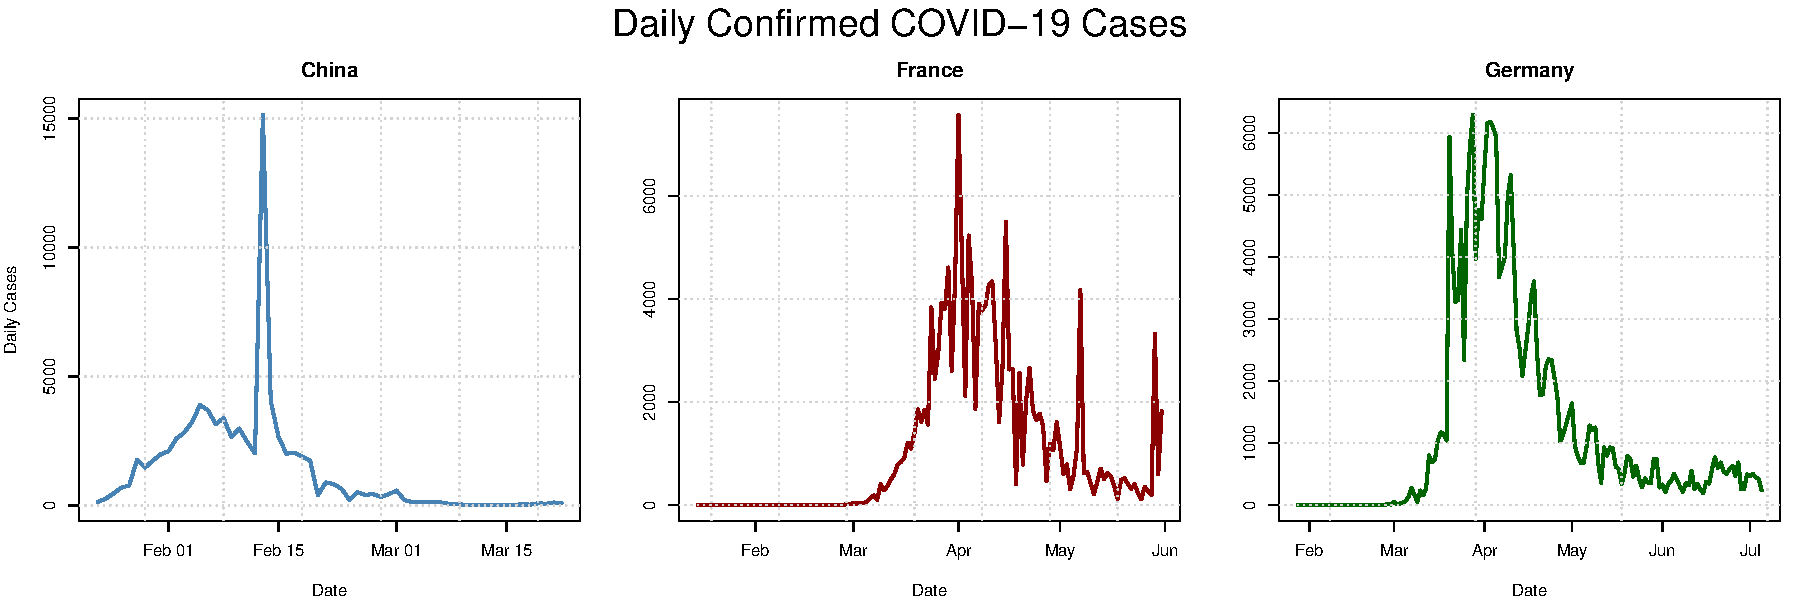
\includegraphics[width=\textwidth]{covid_series_1x3.pdf}
	\caption{Daily confirmed COVID-19 cases in China, France, and Germany (left to right).}
	\label{fig:covid-1x3}
\end{figure}

\subsection{China}
\label{subsec:china}

For China ($L=22$), the selected windows
(Table~\ref{tab:china_entry_exit}) are $[15,26]$, $[15,24]$, $[22,25]$
and $[22,27]$ for $\tau=0.25,0.5,0.75,0.95$, with widths between $3$
and $11$. A window containing $L$ is therefore selected at every
quantile level, but those for $\tau=0.75$ and $\tau=0.95$ begin at $L$
and lie to its right, whereas the others contain $L$ in their
interior. For $\tau=0.5$, the window $[15,24]$ is close to $(14,25)$
reported in~\citet{Der25} under the least-absolute-deviation criterion
for the same dataset.
These results complement the tolerance-based entry-time analysis reported in Supplementary Table~S1: the entry time describes the horizon from which all subsequent estimates remain within the prescribed tolerance, whereas the two-stage construction uses the oscillations of the estimated peak-location path to identify candidate windows for the peak region.

\begin{table}[htbp]
	\centering
	\caption{Retrospective selection of the peak-region candidate for
		COVID-19 in China.
		The selected candidate is the narrowest one with
		$T_{\mathrm{entry}}^{(k)}\le L\le T_{\mathrm{exit}}^{(k)}$.}
	\label{tab:china_entry_exit}
	\begin{tabular}{c|cccccccc}
		\toprule
		$\tau$ &
		$k$ &
		$\epsilon'_k$ &
		$T_{\mathrm{exit}}^{(k)}$ &
		$T_k^*$ &
		$\epsilon_k$ &
		$T_{\mathrm{entry}}^{(k)}$ &
		$w_k$ &
		$L$ \\
		\midrule
		$0.25$ & 1 & 1  & 26 & 15 & 3  & 15 & 11 & 22 \\
		$0.50$ & 2 & 2  & 24 & 15 & 2  & 15 & 9  & 22 \\
		$0.75$ & 1 & 2  & 25 & 22 & 15 & 22 & 3 & 22 \\
		$0.95$ & 3 & 6 & 27 & 26 & 9 & 22 & 5 & 22 \\
		\bottomrule
	\end{tabular}
\end{table}

\subsection{France}
\label{subsec:france}

For France ($L=78$), the selected windows
(Table~\ref{tab:france_entry_exit}) are $[72,79]$, $[71,78]$, $[70,78]$
and $[78,85]$ for $\tau=0.25,0.5,0.75,0.95$, with widths between $7$
and $8$. A window containing $L$ is therefore selected at every
quantile level; only the window for $\tau=0.25$ contains $L$ in its
interior, whereas the others contain $L$ at an endpoint.
These results complement the tolerance-based entry-time analysis reported in Supplementary Table~S2.

\begin{table}[htbp]
	\centering
	\caption{Retrospective selection of the peak-region candidate for
		COVID-19 in France.
		The selected candidate is the narrowest one with
		$T_{\mathrm{entry}}^{(k)}\le L\le T_{\mathrm{exit}}^{(k)}$.}
	\label{tab:france_entry_exit}
	\begin{tabular}{c|cccccccc}
		\toprule
		$\tau$ &
		$k$ &
		$\epsilon'_k$ &
		$T_{\mathrm{exit}}^{(k)}$ &
		$T_k^*$ &
		$\epsilon_k$ &
		$T_{\mathrm{entry}}^{(k)}$ &
		$w_k$ &
		$L$ \\
		\midrule
		$0.25$ & 5 & 13 & 79 & 76 & 13 & 72 & 7  & 78 \\
		$0.50$ & 5 & 10 & 78 & 72 & 11 & 71 & 7 & 78 \\
		$0.75$ & 4 & 10 & 78 & 72 & 11 & 70 & 8 & 78 \\
		$0.95$ & 3 & 5 & 85 & 80 & 6 & 78 & 7 & 78 \\
		\bottomrule
	\end{tabular}
\end{table}

\subsection{Germany}
\label{subsec:germany}

For Germany ($L=61$), the selected windows
(Table~\ref{tab:germany_entry_exit}) are $[60,62]$, $[59,61]$,
$[57,61]$ and $[56,63]$ for $\tau=0.25,0.5,0.75,0.95$, with widths
between $2$ and $7$. A window containing $L$ is therefore selected at
every quantile level; for $\tau=0.5$ and $\tau=0.75$ the window ends at
$L$, whereas the others contain $L$ in their interior.
These results complement the tolerance-based entry-time analysis reported in Supplementary Table~S3.

\begin{table}[htbp]
	\centering
	\caption{Retrospective selection of the peak-region candidate for
		COVID-19 in Germany.
		The selected candidate is the narrowest one with
		$T_{\mathrm{entry}}^{(k)}\le L\le T_{\mathrm{exit}}^{(k)}$.}
	\label{tab:germany_entry_exit}
	\begin{tabular}{c|cccccccc}
		\toprule
		$\tau$ &
		$k$ &
		$\epsilon'_k$ &
		$T_{\mathrm{exit}}^{(k)}$ &
		$T_k^*$ &
		$\epsilon_k$ &
		$T_{\mathrm{entry}}^{(k)}$ &
		$w_k$ &
		$L$ \\
		\midrule
		$0.25$ & 7 & 15 & 62 & 60 & 15 & 60 & 2 & 61 \\
		$0.50$ & 5 & 10 & 61 & 59 & 11 & 59 & 2 & 61 \\
		$0.75$ & 5 & 7 & 61 & 58 & 11 & 57 & 4 & 61 \\
		$0.95$ & 6 & 9  & 63 & 56 & 18 & 56 & 7 & 61 \\
		\bottomrule
	\end{tabular}
\end{table}

\subsection{Admissible candidates $\mathcal K(T)$ on the real data}
\label{subsec:real-K}

For each country and each $\tau$, we apply at every horizon $T$ the
current-horizon construction of Section~\ref{subsec:entry-exit-simulation}
to the path $T\mapsto\hat l(T)$ (Tables~S1--S3 in the supplement).
At the terminal horizon $T=h$ this construction coincides with the
two-stage construction used above. As in the rest of the paper, an
interval $[a,b]$ contains $L$ if $a\le L\le b$; the observed peak day $L$
is $22$, $78$ and $61$ for China, France and Germany.

\paragraph{Size of $\mathcal K(T)$.}
Table~\ref{tab:real_K_terminal} lists $\mathcal K(h)$ and
Table~\ref{tab:real_K_props} gives the proportion of horizons at which
$\mathcal K(T)$ is empty, a singleton, or has at least two elements.
In contrast with the simulations at $\mathrm{SNR}=1000$ and $100$, where
$\mathcal K(T)=\{0\}$ after $T=22$, the set $\mathcal K(T)$ here
typically contains nontrivial candidates ($k\ge1$): its largest size is
$2$ for China and $2$ to $4$ for France and Germany, and its mean size
when nonempty is between $1.1$ and $2.5$. It is empty at many horizons
($31$--$34\%$ for China, $39$--$80\%$ for France and Germany); the
France and Germany grids start later ($T=50$ and $T=40$), so these
proportions are not directly comparable across countries. The real
paths therefore resemble the low-SNR simulations. The rules $\min\mathcal K(T)$
and $\arg\min_k w_k(T)$ select different candidates at
$0$--$38\%$ (China), $0$--$38\%$ (France) and $6$--$50\%$ (Germany) of the
horizons at which an interval is selected.

\begin{table}[htbp]
	\centering
	\small
	\caption{Admissible set $\mathcal K(h)$ at the terminal horizon.}
	\label{tab:real_K_terminal}
	\begin{tabular}{lcccc}
		\toprule
		& $\tau=0.25$ & $\tau=0.50$ & $\tau=0.75$ & $\tau=0.95$ \\
		\midrule
		China ($h=35$)   & $\{1\}$   & $\{2,3\}$ & $\{2,3\}$ & $\{4,5\}$ \\
		France ($h=89$)  & $\{2,3\}$ & $\{3,4\}$ & $\{1\}$   & $\{3,4,5,6\}$ \\
		Germany ($h=75$) & $\{3,4\}$ & $\{3\}$   & $\{1,2\}$ & $\{2,3\}$ \\
		\bottomrule
	\end{tabular}
\end{table}

\begin{table}[htbp]
	\centering
	\small
	\caption{Proportion of horizons with $\mathcal K(T)$ empty, a
		singleton, or with at least two elements, and largest size of
		$\mathcal K(T)$.}
	\label{tab:real_K_props}
	\begin{tabular}{lcccccc}
		\toprule
		Country & $\tau$ & empty & singleton & $\ge2$ & max $|\mathcal K|$
		& mean $|\mathcal K|$ if nonempty \\
		\midrule
		China & 0.25 & 0.31 & 0.63 & 0.06 & 2 & 1.09 \\
		& 0.50 & 0.34 & 0.22 & 0.44 & 2 & 1.67 \\
		& 0.75 & 0.31 & 0.06 & 0.63 & 2 & 1.91 \\
		& 0.95 & 0.34 & 0.13 & 0.53 & 2 & 1.81 \\
		\midrule
		France & 0.25 & 0.68 & 0.10 & 0.23 & 2 & 1.69 \\
		& 0.50 & 0.80 & 0.03 & 0.18 & 2 & 1.88 \\
		& 0.75 & 0.75 & 0.15 & 0.10 & 2 & 1.40 \\
		& 0.95 & 0.80 & 0.08 & 0.13 & 4 & 2.50 \\
		\midrule
		Germany & 0.25 & 0.50 & 0.14 & 0.36 & 2 & 1.72 \\
		& 0.50 & 0.50 & 0.11 & 0.39 & 2 & 1.78 \\
		& 0.75 & 0.50 & 0.11 & 0.39 & 3 & 1.83 \\
		& 0.95 & 0.39 & 0.00 & 0.61 & 4 & 2.36 \\
		\bottomrule
	\end{tabular}
\end{table}

\paragraph{Position of the candidates relative to $L$.}
We examine $\mathcal K(T)$ at $T=L-3$, $L+3$ and $L+10$ (the nearest
available horizons: $19,25,32$ for China, $75,81,88$ for France and
$58,64,71$ for Germany). For $T<L$, every candidate ends at
$T_{\mathrm{exit}}^{(k)}(T)\le T<L$, so no interval can contain $L$;
this is structural, and none does ($0$ of $13$ candidates; $\mathcal K(75)$
is empty for France). For $T>L$, the number of candidates in
$\mathcal K(T)$ whose interval contains $L$, pooled over the
four values of $\tau$, is $3$ of $5$ (China), $1$ of $3$ (France) and
$6$ of $9$ (Germany) at $T=L+3$, and $5$ of $7$, $6$ of $9$ and $6$ of
$9$ at $T=L+10$. Candidates that miss $L$ are mostly narrow and lie on one side of $L$,
near $\hat l(T)$. Table~\ref{tab:real_data_intervals} shows, for each
country and horizon, the narrowest candidate with $k\ge1$, width at most $10$, and
$T_{\mathrm{entry}}^{(k)}\le L\le T_{\mathrm{exit}}^{(k)}$ (ties: smaller $k$,
then smaller $\tau$).
This choice uses $L$ and is illustrative only. Over all horizons $T>L$, the proportion of candidates covering $L$ has no monotone pattern in $k$: for $k=1,2,3,\ge4$ it is $0.82,0.88,0.52,0.42$ (China), $0.25,0.63,0.63,1.00$ (France) and
$0.32,0.64,0.61,0.79$ (Germany). These proportions are descriptive,
since consecutive horizons are dependent.

\begin{table}[htbp]
	\centering
	\small
	\caption{Illustrative candidates: the narrowest $k\ge1$ in
		$\mathcal K(T)$ with width at most $10$ and
		$T_{\mathrm{entry}}^{(k)}\le L\le T_{\mathrm{exit}}^{(k)}$, at $T=L+3$
		and $T=L+10$ ($L=22,78,61$); ties are broken by the smaller $k$,
		then the smaller $\tau$. The last column gives the number of
		candidates in $\mathcal K(T)$, pooled over $\tau$, whose interval
		contains $L$. The selection uses $L$ and is not operational.}
	\label{tab:real_data_intervals}
	\begin{tabular}{lccccccc}
		\toprule
		Country & $T$ & $\tau$ & $k$ & $\widehat l(T)$
		& $[T_{\mathrm{entry}}^{(k)},T_{\mathrm{exit}}^{(k)}]$ & Width
		& Covering $L$ \\
		\midrule
		China   & 25 & 0.50 & 2 & 17 & [15, 22] & 7 & 3 of 5 \\
		China   & 32 & 0.50 & 2 & 17 & [15, 24] & 9 & 5 of 7 \\
		France  & 81 & 0.25 & 2 & 79 & [72, 79] & 7 & 1 of 3 \\
		France  & 88 & 0.95 & 3 & 79 & [78, 85] & 7 & 6 of 9 \\
		Germany & 64 & 0.50 & 1 & 61 & [61, 62] & 1 & 6 of 9 \\
		Germany & 71 & 0.50 & 3 & 64 & [61, 65] & 4 & 6 of 9 \\
		\bottomrule
	\end{tabular}
\end{table}

\paragraph{Operational rule.}
Table~\ref{tab:real_data_minK} gives the interval selected by
$\hat k(T)=\min\mathcal K(T)$ at the same horizons. It contains
$L$ in $4$ of $9$ cases at $T=L+3$ and in $8$ of $12$ at $T=L+10$
($\mathcal K(T)$ is empty in three further cases). Several of these
intervals contain $L$ only at an endpoint (for example $[13,22]$,
$[78,85]$ and $[61,62]$); since the time index is discrete and the
intervals are closed, this is a genuine containment. The candidates of
Table~\ref{tab:real_data_intervals} are not what the operational
rule returns in general: the rule often returns a narrow interval on one
side of $L$. This agrees with the low-SNR simulations, where coverage
of the selected interval was moderate and increased with $T$. These
are single realizations per country, not coverage probabilities.

\begin{table}[htbp]
	\centering
	\small
	\caption{Interval selected by $\hat k(T)=\min\mathcal K(T)$ at
		$T=L+3$ and $T=L+10$. ``Covers $L$'' means
		$T_{\mathrm{entry}}\le L\le T_{\mathrm{exit}}$; a dash means that
		$\mathcal K(T)$ is empty.}
	\label{tab:real_data_minK}
	\begin{tabular}{lcccccccc}
		\toprule
		Country & $T$ & $\tau$ & $\hat k$ & $\widehat l(T)$
		& $[T_{\mathrm{entry}},T_{\mathrm{exit}}]$ & Width & Covers $L$ \\
		\midrule
		China & 25 & 0.25 & 1 & 15 & [14, 15] & 1 & No \\
		& 25 & 0.50 & 1 & 17 & [16, 24] & 8 & Yes \\
		& 25 & 0.75 & 1 & 20 & [13, 22] & 9 & Yes \\
		& 25 & 0.95 & --- & --- & --- & --- & --- \\
		& 32 & 0.25 & 1 & 16 & [15, 26] & 11 & Yes \\
		& 32 & 0.50 & 2 & 17 & [15, 24] & 9 & Yes \\
		& 32 & 0.75 & 2 & 18 & [13, 22] & 9 & Yes \\
		& 32 & 0.95 & 4 & 20 & [13, 26] & 13 & Yes \\
		\midrule
		France & 81 & 0.25 & 1 & 79 & [79, 80] & 1 & No \\
		& 81 & 0.50 & --- & --- & --- & --- & --- \\
		& 81 & 0.75 & 0 & 81 & [80, 81] & 1 & No \\
		& 81 & 0.95 & --- & --- & --- & --- & --- \\
		& 88 & 0.25 & 2 & 82 & [81, 84] & 3 & No \\
		& 88 & 0.50 & 3 & 81 & [73, 82] & 9 & Yes \\
		& 88 & 0.75 & 1 & 81 & [81, 86] & 5 & No \\
		& 88 & 0.95 & 3 & 79 & [78, 85] & 7 & Yes \\
		\midrule
		Germany & 64 & 0.25 & 1 & 62 & [62, 63] & 1 & No \\
		& 64 & 0.50 & 1 & 61 & [61, 62] & 1 & Yes \\
		& 64 & 0.75 & 1 & 60 & [59, 63] & 4 & Yes \\
		& 64 & 0.95 & 2 & 58 & [56, 59] & 3 & No \\
		& 71 & 0.25 & 3 & 65 & [64, 67] & 3 & No \\
		& 71 & 0.50 & 2 & 64 & [61, 66] & 5 & Yes \\
		& 71 & 0.75 & 1 & 65 & [65, 67] & 2 & No \\
		& 71 & 0.95 & 2 & 61 & [60, 65] & 5 & Yes \\
		\bottomrule
	\end{tabular}
\end{table}

\subsection{Entry and exit times with data-driven thresholds}
\label{subsec:real-entry-eps}

The thresholds $\varepsilon=3,5,15$ were chosen by hand. By
Proposition~\ref{prop:ladder}, any $\varepsilon$ selects a rung of the ladder of
the path: $T_{\mathrm{entry}}(\varepsilon)$ is an exit time
$T_{\mathrm{exit}}^{(k+1)}(h)$ plus one. For China and $\varepsilon=3$, the
values $15,13,23,28$ obtained for $\tau=0.25,0.5,0.75,0.95$ correspond to
$k+1=3,4,2,3$; for $\tau=0.75$, every $\varepsilon\in[2,17)$ gives the same
value $23$. For $\varepsilon=0$, the start of the final plateau is
$T_{\mathrm{entry}}(0)=27,30,26,31$ for China, $86,89,87,88$ for France and
$73,74,74,74$ for Germany ($\tau=0.25,0.5,0.75,0.95$).

The two-stage construction suggests data-driven levels instead:
$(\varepsilon,\varepsilon')=(\epsilon_k,\epsilon'_k)$ for a candidate $k$,
with $\epsilon_k\ge\epsilon'_k$. We use them as a diagnostic, not as a
replacement for the two-stage windows.
Table~\ref{tab:tentry_eps_retro} compares the pair
$[T_{\mathrm{entry}}(\epsilon_k;h),T_{\mathrm{exit}}(\epsilon'_k;h)]$ with
the two-stage window for the retrospectively selected candidate (the
narrowest one containing $L$,
Tables~\ref{tab:china_entry_exit}--\ref{tab:germany_entry_exit}); the
corresponding table for the operational candidate $\hat k(h)=\min\mathcal K(h)$
is Table~\ref{tab:tentry_eps_oper}.

\begin{table}[htbp]
	\centering
	\small
	\caption{Two-stage window and threshold-based window with
		$(\varepsilon,\varepsilon')=(\epsilon_k,\epsilon'_k)$ at $T=h$, for
		the retrospectively selected candidate $k$. The last column is 
		$T_{\mathrm{entry}}(\varepsilon; h)$ with
		$\varepsilon=3,5,15$ for China, France and Germany.}
	\label{tab:tentry_eps_retro}
	\begin{tabular}{lccccc c}
		\toprule
		Country & $\tau$ & $k$ & $(\epsilon_k,\epsilon'_k)$
		& $[T_{\mathrm{entry}}^{(k)},T_{\mathrm{exit}}^{(k)}]$
		& $[T_{\mathrm{entry}}(\epsilon_k;h),T_{\mathrm{exit}}(\epsilon'_k;h)]$
		& $T_{\mathrm{entry}}(\varepsilon)$ \\
		\midrule
		China ($L=22$)    & 0.25 & 1 & (3, 1)   & [15, 26] & [15, 16] & 15 \\
		& 0.50 & 2 & (2, 2)   & [15, 24] & [23, 23] & 13 \\
		& 0.75 & 1 & (15, 2)  & [22, 25] & [23, 23] & 23 \\
		& 0.95 & 3 & (9, 6)   & [22, 27] & [27, 27] & 28 \\
		\midrule
		France ($L=78$)   & 0.25 & 5 & (13, 13) & [72, 79] & [79, 79] & 85 \\
		& 0.50 & 5 & (11, 10) & [71, 78] & [71, 73] & 82 \\
		& 0.75 & 4 & (11, 10) & [70, 78] & [70, 73] & 80 \\
		& 0.95 & 3 & (6, 5)   & [78, 85] & [85, 85] & 85 \\
		\midrule
		Germany ($L=61$)  & 0.25 & 7 & (15, 15) & [60, 62] & [60, 60] & 60 \\
		& 0.50 & 5 & (11, 10) & [59, 61] & [61, 61] & 59 \\
		& 0.75 & 5 & (11, 7)  & [57, 61] & [57, 59] & 56 \\
		& 0.95 & 6 & (18, 9)  & [56, 63] & [56, 60] & 57 \\
		\bottomrule
	\end{tabular}
\end{table}

By Proposition~\ref{prop:ladder}(iii), $T_{\mathrm{entry}}(\epsilon_k;h)\ge
T_{\mathrm{entry}}^{(k)}$ in all cases: the two-stage entry time measures
the oscillation up to $T_{\mathrm{exit}}^{(k)}$, the threshold-based one up
to $h$. The two coincide in $6$ of $12$ cases for each selection. For the
exit times, Proposition~\ref{prop:ladder}(i) gives
$T_{\mathrm{exit}}(\epsilon'_k;h)=T_{\mathrm{entry}}(\epsilon'_k;h)
=T_{\mathrm{exit}}^{(k+1)}(h)+1\le T_{\mathrm{exit}}^{(k)}(h)$, with equality
exactly when rung $k$ of the ladder reduces to a single horizon. This
happens in $4$ of $12$ cases for the retrospective selection (China
$\tau=0.95$, France $\tau=0.25,0.95$, Germany $\tau=0.5$) and in $6$ of
$12$ for the operational one (China $\tau=0.75$, France $\tau=0.5,0.95$,
Germany $\tau=0.25,0.5,0.75$). The condition $\epsilon_k>\epsilon'_k$ holds
in $9$ of $12$ cases (retrospective) and $8$ of $12$ (operational); when
$\epsilon_k=\epsilon'_k$, $T_{\mathrm{exit}}(\epsilon'_k;h)=
T_{\mathrm{entry}}(\epsilon_k;h)$ and the pair reduces to a single horizon.

The threshold-based windows contain $L$ in only $1$ of $12$ cases for the
retrospective selection (Germany, $\tau=0.5$) and in $3$ of $12$ for the
operational one (China $\tau=0.75,0.95$, Germany $\tau=0.5$), always at an
endpoint, whereas the two-stage windows contain $L$ in $12$ of $12$ cases
(by construction) and $8$ of $12$ cases, respectively. The pair
$(\epsilon_k,\epsilon'_k)$ therefore does not reproduce the two-stage
window; it indicates instead the scale of threshold that the path itself
suggests. For Germany, $\epsilon_k$ ($15,11,11,18$) is of the same order as
$\varepsilon=15$; for China it is close to $\varepsilon=3$ at
$\tau=0.25,0.5$ ($3,2$) but three to five times larger at
$\tau=0.75,0.95$ ($15,9$); for France it exceeds $\varepsilon=5$
($13,11,11,6$). Accordingly, $T_{\mathrm{entry}}(\epsilon_k;h)$ coincides
with $T_{\mathrm{entry}}(\varepsilon;h)$, $\varepsilon=3,5,15$, in $4$ of
$12$ cases and is earlier in three of the four French cases
($79,71,70$ against $85,82,80$ for $\tau=0.25,0.5,0.75$). These
comparisons are descriptive: they rest on a single realization per
country, and the retrospective selection uses the observed peak $L$.

\begin{table}[htbp]
	\centering
	\small
	\caption{Same as Table~\ref{tab:tentry_eps_retro} for the operational
		candidate $\hat k(h)=\min\mathcal K(h)$.}
	\label{tab:tentry_eps_oper}
	\begin{tabular}{lccccc c}
		\toprule
		Country & $\tau$ & $\hat k$ & $(\epsilon_{\hat k},\epsilon'_{\hat k})$
		& $[T_{\mathrm{entry}}^{(\hat k)},T_{\mathrm{exit}}^{(\hat k)}]$
		& $[T_{\mathrm{entry}}(\epsilon_{\hat k};h),T_{\mathrm{exit}}(\epsilon'_{\hat k};h)]$
		& $T_{\mathrm{entry}}(\varepsilon)$ \\
		\midrule
		China ($L=22$)    & 0.25 & 1 & (3, 1)   & [15, 26] & [15, 16] & 15 \\
		& 0.50 & 2 & (2, 2)   & [15, 24] & [23, 23] & 13 \\
		& 0.75 & 2 & (20, 17) & [13, 22] & [13, 22] & 23 \\
		& 0.95 & 4 & (21, 15) & [13, 26] & [13, 22] & 28 \\
		\midrule
		France ($L=78$)   & 0.25 & 2 & (7, 6)   & [81, 84] & [81, 83] & 85 \\
		& 0.50 & 3 & (6, 4)   & [73, 82] & [82, 82] & 82 \\
		& 0.75 & 1 & (2, 2)   & [81, 86] & [81, 81] & 80 \\
		& 0.95 & 3 & (6, 5)   & [78, 85] & [85, 85] & 85 \\
		\midrule
		Germany ($L=61$)  & 0.25 & 3 & (7, 7)   & [66, 68] & [68, 68] & 60 \\
		& 0.50 & 3 & (10, 3)  & [61, 66] & [61, 66] & 59 \\
		& 0.75 & 1 & (1, 1)   & [66, 73] & [73, 73] & 56 \\
		& 0.95 & 2 & (6, 5)   & [59, 72] & [66, 67] & 57 \\
		\bottomrule
	\end{tabular}
\end{table}

\section{Conclusion}
\label{sec:conclusion}

This paper develops a quantile-based framework for predicting the
location of a peak in a Gaussian-shaped time series observed sequentially
and corrupted by additive noise. For fixed candidate values of the
peak location and spread, the amplitude estimator is characterized as
a weighted $\tau$-quantile of a transformed version of the observations.
We adopt a $\tau$-aligned asymmetric Laplace working model, whose
negative log-likelihood is proportional to the quantile check loss, to
calibrate the noise in the simulations and to relate the estimation
criterion to a likelihood formulation.

We also investigate the evolution of the estimated peak location as
the observation horizon increases. The stabilization time describes
when the sequential estimate becomes constant over the remaining
horizon, subject to a minimum plateau-length condition. The simulations
show that this criterion is informative when the signal-to-noise ratio
is high or moderate, but becomes less reliable under substantial noise.
To address situations in which the point estimate does not stabilize
early enough, we introduce a two-stage construction of candidate
entry--exit intervals based on the oscillations of the estimation
trajectory. The operational selection rule uses the current point
estimate and does not require knowledge of the true peak location.
The oscillation function has a ladder structure
(Proposition~\ref{prop:ladder}): a tolerance-based entry time is an exit time of the two-stage construction plus one, and, whenever the final plateau contains at least \(m\) horizons, the stabilization time coincides with the entry time at tolerance zero.
On the COVID-19 data,
taking the levels $(\epsilon_k,\epsilon'_k)$ of the two-stage construction
as thresholds does not reproduce the two-stage windows, but it indicates
the scale of tolerance suggested by the estimated path.

The Monte Carlo experiments show that the performance of the selected
intervals depends strongly on the signal-to-noise ratio. Under the
high- and moderate-SNR settings considered, the selected intervals
achieve full empirical coverage in the simulated replicates once the
peak becomes identifiable. Under low SNR, intervals can be selected
early without containing the true peak, although empirical coverage
generally improves as more observations become available. These results
also illustrate that a high interval-selection rate does not necessarily
imply high coverage. The application to daily COVID-19 cases in China,
France, and Germany demonstrates how the proposed construction can be
applied to real sequential estimation trajectories. The real-data
results also show that the admissible candidate set may be empty at
some horizons and that the operationally selected interval need not
contain the retrospectively observed peak.

Several limitations suggest directions for further research. The
analysis is based on a Gaussian-shaped peak and a specified
$\tau$-aligned noise model, so performance under more complex peak
shapes, multiple peaks, temporal dependence, or model misspecification
requires further investigation. Moreover, the entry--exit intervals
are data-driven interval estimates rather than confidence intervals
with guaranteed nominal coverage. Establishing theoretical coverage
properties, and developing selection rules that balance interval width,
coverage, and the possibility that no interval is selected, are
important topics for future work.

\bibliography{references}

\paragraph*{Data Availability Statement}

The daily COVID-19 case counts analyzed in Section~7 are derived
from two publicly available sources. The Chinese series is obtained
from the Johns Hopkins University Center for Systems Science and
Engineering (JHU CSSE) feed through the \texttt{COVID19} R package,
covering the period 22 January to 22 March 2020. The French and
German series are obtained from the European Centre for Disease
Prevention and Control (ECDC) open data portal, covering the periods
15 January to 31 May 2020 and 28 January to 5 July 2020,
respectively. All data used in this study are publicly available at
the sources cited above and in the bibliography.

%\paragraph*{Conflict of Interest Statement}
%
%The authors declare no conflict of interest.
%
%\paragraph*{Funding Statement}
%
%This research did not receive any specific grant from funding
%agencies in the public, commercial, or not-for-profit sectors.
%
%\paragraph*{Supplementary material}
%The appendix and additional material are provided in a separate Supplementary document.

\paragraph*{Declaration of generative AI}
During the preparation of this work the authors used Claude (Anthropic) in order
to improve the language and clarity of the text, and to suggest wording for some passages. 
After using this tool, the authors reviewed and edited the content as needed and
take full responsibility for the content of the published article.

\end{document}